%For arxiv submission
\documentclass[useAMS, usenatbib]{mnras}
\usepackage{graphicx,amsmath,color,amssymb}
%\voffset=-0.8in
%MNRAS
%\documentclass[useAMS, usenatbib, usegraphicx, twocolumn]{mnras}

%[YAH commented out, my editor didn't like it...]
\usepackage[pdftitle={A hybrid particle-analytic method for non-linear neutrino structure}, draft]{hyperref}

% \newcommand{\eprint}[1]{\href{http://arxiv.org/abs/#1}{#1}}
% \newcommand{\adsurl}[1]{\href{#1}{ADS}}


\topmargin -1.5cm
\bibliographystyle{mnras}

\newcommand{\beq}{\begin{equation}}
\newcommand{\eeq}{\end{equation}}
\newcommand{\barr}{\begin{eqnarray}}
\newcommand{\earr}{\end{eqnarray}}

\newcommand{\rme}{\textrm{e}}
\newcommand{\rmH}{\textrm{H}}
\newcommand{\Ly}{\textrm{Ly}}
\newcommand{\pabn}{p_{\textrm{ab}}^n}
\newcommand{\pscn}{p_{\textrm{sc}}^n}
\newcommand{\rmd}{\textrm{d}}
\newcommand{\N}{\mathcal{N}}
\newcommand{\nuc}{\nu_{\rm c}}
\newcommand{\Tm}{T_{\rm m}}
\newcommand{\Tr}{T_{\rm r}}
\newcommand{\nh}{n_{\rm H}}
\newcommand{\bfA}{\boldsymbol{A}}
\newcommand{\bfr}{\boldsymbol{r}}
\newcommand{\bfV}{\boldsymbol{V}}
\newcommand{\bs}{\boldsymbol}
\newcommand{\mH}{\mathcal{H}}

\newcommand{\natu}{Nature (London)}
\newcommand{\aas}{Bull. Am. Astron. Soc.}
\newcommand{\gadget}{{\small GADGET\,}}

\newcommand{\spb}[1]{{\textcolor{green}{[{\bf SPB}: #1]}}}
\newcommand{\yah}[1]{{\textcolor{blue}{[{\bf YAH}: #1]}}}

\newcommand{\Mpch}{\,\mathrm{Mpc} \,h^{-1}}
\newcommand{\hMpc}{h^{-1}\,\mathrm{Mpc}}
\newcommand{\Lya}{Lyman-$\alpha\;$}
%%%%%%%%%%%%%%%%%%%%%%%%%%%%%%%%%%%%%%%%%%%%%%%%%%%%%%%%%%%%%%%%%%%%%%%%%%%%%%%%%%%%%%%%%%%%%%%%%%


\begin{document}

\title{An Efficient and Accurate Hybrid Method for Simulating Non-Linear Neutrino Structure}
\author[ S. Bird et al.]{Simeon Bird$^1$\thanks{E-mail: sbird@ucr.edu}, Yacine Ali-Ha\"{\i}moud$^2$, Yu Feng$^3$, Jia Liu$^4$\vspace{1.5mm}\\
$^1$UC Riverside, Riverside, CA  and Johns Hopkins University, Baltimore, MD\\
$^2$Center for Cosmology and Particle Physics, Department of Physics,
New York University, New York, NY\\
$^3$Institution\\
$^4$Institution}

\date{\today}

\pagerange{\pageref{firstpage}--\pageref{lastpage}} \pubyear{2012}
\pagenumbering{arabic}
\label{firstpage}

\maketitle

\begin{abstract}
We present an improved method for simulating massive neutrinos in cosmological structure formation simulations, together with an easy to use public implementation.
Our method builds on our earlier linear response approximation, and preserves its good behaviour at early times and in the linear regime, while better following the non-linear clustering of neutrinos on small scales. Massive neutrinos are split into initially ``fast'' and ``slow'' components. The fast component is followed with a modified linear response approximation, which solves the linearized Boltzmann equation analytically. The slow component, which may cluster non-linearly, is followed using neutrino particles included in the initial conditions. Until a neutrino switch-on time, these particles act as passive tracers, thus avoiding the worst effects of particle shot noise. We show that our hybrid method matches (and for small neutrino masses, exceeds) the accuracy of neutrino particle simulations with substantially lower particle load.
\end{abstract}

\begin{keywords}
        neutrinos - cosmology: large-scale structure of Universe - cosmology: dark matter
\end{keywords}

\section{Introduction}

%Neutrinos have mass. Neutrino mass is important because. Neutrinos affect structure. In order to measure the mass accurately with structure we need to know precisely how neutrinos affect structure.
%The structure in question is non-linear structure. We thus need to run simulations. This paper is about a method to put neutrinos into structure simulations.
Neutrinos are the lightest standard model particles, and neutrino oscillation experiments have shown that the sum of the neutrino masses is $M_\nu > 0.06$ eV \citep{Becker-Szendy_1992, Fukuda_1998}.
However, measuring the neutrino mass in the laboratory is challenging due to the large difference in mass scales between neutrinos and other standard model particles \cite[although see][]{Wolf_2010}.

However, massive neutrinos %in the cosmic neutrino background
also affect the growth of large-scale structure. They behave as light thermal relics, suppressing clustering below their thermal
free-streaming length \citep[e.g.][]{Lesgourgues_2006, Wong_2011}.
Measurements of the clustering of matter and matter tracers in the Universe can detect this effect and thus constrain the total mass of neutrinos.

Cosmological constraints on the neutrino mass sum $M_\nu$ are quickly approaching the lower limit implied by neutrino oscillation data. For example, the Planck team obtained a 95 \% CL upper limit of $M_\nu<0.23$~eV~\citep{planck2015xiii} using primary cosmic microwave background (CMB) temperature data, combined with low-$\ell$ polarization, CMB lensing, type Ia supernovae~\citep{Betoule_2014}, and baryon acoustic oscillation
measurements~\citep{Beutler_2011, Anderson_2014, Ross_2015}. \cite{Palanque_2015} found a tighter constraint of $M_\nu<0.15$~eV by adding Lyman-$\alpha$ forest data from the Sloan Digital Sky Survey (SDSS). However, recent weak-lensing data from the Dark Energy Survey combined with Planck weakens the upper limit to $0.29$ eV \citep{DES_2017}, and the most recent galaxy power spectrum measurements from SDSS show a slight preference for a non-zero neutrino mass of $M_\nu = 0.3$ eV \citep{Beutler_2014}.
%Not citing HSC or KIDS because they are not yet competitive neutrino mass constraints \citep{HSC_2017}.
% Taken together, these experiments indicate that a detection of neutrino mass from cosmology is imminent. However, realizing the statistical power of future surveys will require extremely accurate modelling
%of structure growth.
Near-future large cosmological surveys such as the Dark Energy Spectroscopic Instrument (DESI) \citep{DESI} or the
Large Synoptic Survey Telescope~(LSST) \citep{LSST, Joudaki_2012} will have the statistical power to measure the neutrino mass even if it is close to $0.06$ eV, the minimum required by oscillation experiments \citep{Abazajian_2015}.

Realizing the statistical power of future surveys will require extremely accurate modelling of structure growth and the effects of massive neutrinos on the matter density field.
Furthermore, current and future experiments achieve their statistical power from small scales where structure formation is in the non-linear regime \citep[e.g.~][]{Troxel_2017, HSC_2017}.
As following structure growth on non-linear scales ultimately requires fitting to $N$-body cosmological simulations, there is an urgent need to incorporate massive neutrinos into cosmological structure simulations
in a way both accurate and computationally inexpensive.
If the simulation methods used are insufficiently accurate, experiments will measure incorrect values for the neutrino mass.
Conversely, if simulation techniques are overly computationally intensive, the number of simulations which can be performed will be reduced, again impeding the accuracy of the cosmological parameter measurement.

The standard approach to include massive neutrinos in structure-formation simulation has been to use the $N$-body method, which consists in solving for the evolution of discrete phase-space chunks or ``particles", akin to those used for CDM, but with a %lower particle mass and a
large thermal velocity imposed in the initial conditions. This approach has been used extensively in the past, \cite[e.g.~][]{Brandbyge_2008, Bird_2012, Inman_2017, FVN_2017}. Its main advantages are that it is simple to implement and fully includes non-linear clustering of neutrinos\footnote{Although note that the small-scale tree force for the neutrino particles is often disabled in previous works.}. It has been used to examine voids \citep{Massara_2015}, clusters and halos \citep{FVN_2014, Castorina_2014, Costanzi_2013}, large-scale clustering \citep{Castorina_2015} and the ISW effect \citep{Carbone_2016}.

On the flip side, particle neutrinos are computationally expensive and can suffer from a variety of numerical problems related to their initially large thermal velocities. For instance, fast neutrino particles frequently move between processors in a parallel code, limiting scalability. In addition, for $M_\nu$ close to its floor, properly modelling the splitting between neutrino mass states involves the use of at least two particle species, hence requiring more particles. Perhaps the most acute issue is that of shot noise, which dominates over the small intrinsic perturbations of the neutrino fluid at early times and on small scales. %due the finite number of neutrino particles
% and their random distribution, induces shot noise power $P \propto 1/N_\mathrm{part}$ at early times, which can only be reduced by a large particle load.
A variety of techniques have been proposed to reduce neutrino shot noise in the $N$-body technique. The most obvious but no less technically challenging approach is to massively increase the number of neutrino particles, to which the shot noise is inversely proportional; for instance, \cite{Emberson_17} simulated a total of 2.97 trillion particles. Another approach, proposed by \cite{Banerjee_2016}, is to use smoothed particle hydrodynamics to evolve the neutrino continuity and momentum equations, and simultaneously evolve particle neutrinos from which the stress tensor is extracted. Finally, \cite{Banerjee_2018} recently pointed out that the shot noise can be considerably reduced by densely sampling the full neutrino velocity distribution at each grid point, rather than assigning a single particle with a randomly drawn velocity.

%We find that achieving $1\%$ convergence in the matter power spectrum requires $1024^3$ neutrino particles for a neutrino mass $M_\nu = 0.4$ eV. The effects of shot noise can be reduced by initialising the simulation at a lower redshift (e.g.~$z=49$ for $M_\nu = 0.4$ eV), but this limits the accuracy of the CDM growth function. Furthermore, in a parallel code the large thermal velocities of the neutrinos causes particles to frequently move between processors, limiting scalability. Finally, the particle approximation limits the physics that can be implemented. Modelling the splitting between neutrino mass states involves the use of at least two particle species.

While these techniques are successful in reducing shot noise, they always involve a significant additional computational cost. An orthogonal route that has been explored is to rely on perturbation theory to model massive neutrinos. For instance, \cite{Brandbyge_2009} use the transfer function of neutrinos computed in linear theory to compute their overdensity on a grid. In the same spirit, \cite{AHB}, hereafter AHB13, proposed modelling neutrinos using the linear-response approximation \citep{Bond_1980, Ma_1994}. This is more accurate than pure linear theory, as it accounts for the full non-linear CDM potential to which neutrinos respond, and correctly models the phases of the neutrino overdensity, at no additional computational cost.
%The neutrino component is followed using first-order linear perturbation theory, clustering in a background potential generated from the fully non-linear clustering of the CDM particles. The main improvement of this method over earlier perturbation-based neutrino codes \citep{Brandbyge_2009} was the use of the full non-linear CDM potential. This makes it possible to achieve accurate results for any level of CDM clustering, as long as the neutrino free-streaming scale is larger than the non-linear scale.
AHB13 showed that the linear-response approximation (hereafter, LRA) accurately describes the effect of massive neutrinos on the growth of cold dark matter (CDM), computing the matter power spectrum $P(k)$ at $ < 0.2\%$ accuracy for $M_\nu < 0.6$ eV. Due to its minimal computational overhead relative to a pure CDM simulation, it has been used to investigate the combined effects of massive neutrinos and baryons \citep{Mummery_2017} and to constrain the neutrino mass using hydrodynamic simulations of large-scale structure \citep{McCarthy_2018, McCarthy_2017}.

The implementation of the LRA in AHB13 is applied to \emph{all} neutrinos, regardless of their initial thermal velocity. AHB13 found that, for $M_\nu \gtrsim 0.3$ eV and $z \lesssim 0.5$, this method under-estimates the clustering of neutrinos relative to what is found in particle simulations, even though their characteristic overdensity is significantly less than unity on all scales. This can be understood qualitatively as follows: the LRA is formally the first order of an expansion in $\phi/v^2$, and is increasingly inaccurate for particles with low initial velocity $v$. As the initial velocity of neutrinos follows a Fermi-Dirac distribution, there are always neutrinos that are slow enough to cluster non-linearly. These neutrinos can dominate the clustering on small scales, even if they are a small fraction of the neutrino matter density, because linear growth is highly suppressed. %\spb{Does the above rephrasing work for you?}

In this paper, we present an improved implementation of the LRA, allowing us to not only model the CDM but also the clustering of neutrinos themselves.  %extension of the linear-response method which allows to accurately model neutrinos with low initial velocities, and thus reproduce the neutrino power spectrum from particle simulations.
As in AHB13, we model all neutrinos with the LRA, but only down to a cutoff redshift $z_\nu \approx 1$. Later on, neutrinos are split by their initial velocity into a fast and a slow components. The LRA is applied only to the fast component, while the slow component is followed using neutrino particles. The slow initial velocity of our particle neutrinos mitigates the numerical problems that plague purely particle simulations. Our new method allows a single simulation code to produce a well-converged neutrino simulation, at any neutrino mass, which includes late-time non-linear growth in the neutrino sector. %We describe it in more detail in Section~\ref{sec:hybrid}.
We provide an improved public implementation of our neutrino simulation
method\footnote{The latest version may be found here: \url{https://github.com/sbird/kspace-neutrinos/}}.
While the implementation in AHB13 was tied to \gadget \citep{Springel_2005}, our new version is adaptable to a variety of structure simulation codes. We also include patches for Gadget-2 \citep{Springel_2005}, which were used for a large suite of simulations in \cite{Liu_2017}.

This article is organized as follows. In Section \ref{sec:lin_resp}, we review the linear-response approximation, and study its regime of validity in detail. We describe our hybrid method to simulate neutrinos in Section \ref{sec:hybrid} and our suite of simulations in Section \ref{sec:simulations}. We describe our results and compare different methods in Section \ref{sec:results}. We conclude in Section \ref{sec:conclusion}. Appendix \ref{sec:manual} is a user's manual for our neutrino module. In appendix \ref{sec:initcond} we describe improvements to our initial conditions since AHB13.


\section{Linear-response approximation} \label{sec:lin_resp}


%\subsection{Analytic Neutrinos}
%\label{sec:analytic}
%
%
%In this section we describe the semi-analytic linear response method for treating neutrinos from \cite{AHB}.
%Motivated by the numerical difficulties with particle simulations, we sought to use an analytic treatment.
%The applicability of this method follows is because neutrinos do not cluster below their free-streaming length, given by
%\begin{equation}
% k_{\rm fs}(z) \approx \frac{0.08}{\sqrt{1+z}}
%\sqrt{\frac{\Omega_{\rm M}}{0.3}} \frac{m_{\nu}}{0.1 ~ \textrm{eV}} h~ \textrm{Mpc}^{-1}.
%\label{eq:kfs}
%\end{equation}
%For astrophysically relevant neutrino masses, this free-streaming length is larger than the non-linear scale.
%Thus while CDM exhibits strong non-linear clustering, the neutrino species does not, behaving
%almost as expected from linear perturbation theory. However, the neutrino species does exhibit increased clustering
%as a result of the deeper non-linear CDM potential. The method of \cite{AHB} is thus a linear response,
%in which the neutrino linear theory perturbation grows due as a result of the non-linear growth of CDM.
%
%The neutrino power-spectrum is then given by (eq. (63) of \cite{AHB})
%\begin{align}
%P_{\nu}^{1/2}(k, \tau) &= \mathcal{I}_{s_i, s}
%P_{\nu}^{1/2}(k, \tau_i) \left\{1 - (s - s_i)  a_i [\theta_{\nu}/\delta_{\nu}]_{i}(k)\right\}\nonumber\\
%&+ \frac32 \Omega_{\rm M} H_0^2 \int_{\tau_i}^{\tau} \mathcal{I}_{s', s}
%P^{1/2}_{\rm M}(k, \tau') (s - s')d \tau', \label{eq:P-final}
%\end{align}
%where $\mathcal{I}_{s_1, s_2} \equiv \mathcal{I}([s_2 -s_1]k/m)$. $\mathcal{I}$ is defined to be
%the Fourier transform of the unperturbed neutrino distribution function in momentum space, normalized so
%that $\mathcal{I}(0) = 1$ \citep{Brandenberger_1987, Bertschinger_Watts_1988},
%\begin{equation}
%\mathcal{I}[X; f^0] \equiv \frac{\int dq~ j_0(q X) q^2 f^0(q) }{\int dq ~q^2 f^0(q)}. \label{eq:I.def}
%\end{equation}
%
%The first term of Eq.~\ref{eq:P-final} represents a contribution from the initial conditions. In practice
%for astrophysical masses neutrinos are initially relativistic, so this term is extremely small and may
%be safely neglected (although we include it in our implementation for completeness).
%The second term is the perturbation to a neutrino geodesic from the CDM potential
%integrated over cosmic time. Our implementation computes the matter power spectrum for every PM timestep
%and stores it in a table, evenly spaced in $\Delta a = 0.01$\footnote{The code actually provides the CDM power spectrum.
%We estimate the matter power spectrum by adding the neutrino power from the previous timestep. It would be possible
%to iterate this procedure, but in practice it is always immediately converged to a high degree of accuracy.}.
%The neutrino power spectrum is computed by performing an integral over all past matter power spectra, interpolated in log space.
%
%Eq.~\ref{eq:P-final} computes the neutrino power spectrum from stored CDM power spectra.
%A computation of the neutrino potential would use the CDM potential over all of cosmic history, which is impractical
%to store at the required number of time slices. We make the approximation that neutrinos and
%have a cross-correlation coefficient of unity. Thus, in order to recover the neutrino potential, we use
%\begin{equation}
%\delta_{\nu}(\bs k, \tau) = \left(\frac{P_{\nu}(k,
%    \tau)}{P_{\rm cdm}(k, \tau)}\right)^{1/2} \delta_{\rm cdm}(\bs k, \tau).\label{eq:phases}
%\end{equation}
%Equivalently, we assume that the neutrinos and CDM have identical Fourier phases or that neutrinos perfectly trace CDM structure.
%Physically, this is plausible: neutrinos behave much like CDM on scales larger than their free streaming length,
%and do not cluster on smaller scales (so any differences in their phases has limited practical impact, as $\delta_\nu$ is zero).
%Figure~\ref{fig:cross-corr} shows the cross-correlation coefficient,
%\begin{equation}
%R = \frac{\left\langle \delta_\nu \delta_\mathrm{cdm} \right\rangle}{\sqrt{P_{\rm{cdm}} P_{\rm{\nu}}}}
%\end{equation}
%between neutrinos and CDM from a neutrino particle simulation. It is indeed unity on large scales,
%dropping to zero on small scales where the particle neutrino power is dominated by shot noise.
%


The linear-response approximation (herafter, LRA), sometimes referred to as the \cite{Gilbert_1966} approximation, consists of linearizing the collisionless Boltzmann equation for neutrinos in the gravitational interaction. Formally, the LRA is the first order of an expansion in $\phi/v^2$, where $v^2$ is the variance of the velocity distribution. This implies that it is only well defined for \emph{hot} species, and is not adapted to standard cold dark matter \citep{YAH_15}. It is equivalent to assuming nearly-straight-line trajectories, with small deflections of order $\phi/v^2$. The LRA was first applied to cosmological neutrinos in the linear regime by \cite{Bond_Szalay_1983} and \cite{Brandenberger_1987}, and by several authors since then \citep{Singh_Ma_2003, Ringwald_Wong_2004}. In AHB13, the LRA was integrated into an N-body code and applied to the entire neutrino distribution. As the linear response in this case is to the non-linear Newtonian potential of the cold dark matter, it is possible to obtain the neutrino potential even in the non-linear regime of structure formation. In this section we review this approximation and study its regime of validity.

\subsection{General equations}

We start by briefly reviewing the LRA for a general collisionless species with phase-space density $f$. We work in the deep sub-horizon limit, in the conformal Newtonian gauge \citep{Ma_1995}. We denote by $s$ the ``superconformal'' time $(ds \equiv dt/a^2$, where $a$ is the scale factor), and overdots denote derivatives with respect to $s$. Comoving scales are denoted by $\bs{x}$ and $\bs{u} \equiv \dot{\bs{x}}$ denotes the rescaled peculiar velocity of a massive particle. We normalize the phase-space density such that the overdensity is given by
\beq
1 + \delta(s, \bs{x}) = \int d^3 u ~ f(s, \bs{x}, \bs{u}).
\eeq
For a non-relativistic particle, the geodesic equation is $\dot{\bs{u}} = - a^2  \bs{\nabla}_{\bs{x}} \phi$, where $\phi$ is the Newtonian potential. The phase-space density is conserved along trajectories, as is encoded by the collisionless Boltzmann (or Vlasov) equation
\beq
\dot{f} + \bs{u} \cdot \bs{\nabla}_{\bs{x}} f - a^2 \bs{\nabla}_{\bs{x}} \phi \cdot \bs{\nabla}_{\bs{u}} f = 0. \label{eq:Vlasov}
\eeq
%The particle or $N$-body method solves the Vlasov equation numerically by effectively discretizing $f$.
The linear-response method consists in solving for $f$ to linear order in the gravitational potential. Specifically, it is the first order in an expansion in the small parameter $\epsilon \sim a^2 \phi/u^2$. We denote by $f^0(\bs{u})$ the unperturbed, homogenous (but not necessarily isotropic) phase-space density, which integrates to unity. Linearizing Eq.~\eqref{eq:Vlasov} and taking its Fourier transform, we get, denoting by $\bs{k}$ the comoving wavenumber,
\beq
\dot{f} + i (\bs{k} \cdot \bs{u}) f = i a^2 \phi ~ \bs{k} \cdot \bs{\nabla}_{\bs{u}} f^0. \label{eq:Boltz-Fourier}
\eeq
Given initial conditions at $s_i$, this has an explicit integral solution,
\barr
f(s, \bs{k}, \bs{u}) &=& \rme^{- i(\bs{k} \cdot \bs{u}) (s - s_i)} f(s_i, \bs{k}, \bs{u}) \nonumber\\
&+& i \bs{k} \cdot \bs{\nabla}_{\bs{u}} f^0 \int_{s_i}^s d s' \rme^{- i \bs{k} \cdot \bs{u} (s - s')} a'^2 \phi(s', \bs{k}).~~~
\earr
The overdensity is then obtained by integrating over velocities. Using Poisson's equation, $k^2 \phi = - \frac32 H_0^2 \Omega_M a^{-1} \delta_M$, where $\delta_M$ is the total matter overdensity, we arrive at
\barr
\delta(s, \bs{k}) &=& \delta_{\rm I}(s,s_i, \bs{k})\nonumber\\
&+& \frac32 H_0^2 \Omega_M \int_{s_i}^s d s' (s-s') \mathcal{I}[\bs{k}(s-s')] a' \delta_M(s', \bs{k}), ~~~~\label{eq:delta-phi}
\earr
where the first piece corresponds to the propagation of initial perturbations from $s_i$ to $s$, and the kernel $\mathcal{I}$ is the Fourier transform of the unperturbed phase-space density \citep{Brandenberger_1987, Bertschinger_Watts_1988}:
\barr
\mathcal{I}(\bs{k}\Delta s ) % &\equiv& - \frac{i}{k^2 \Delta s} \int d^3 u  ~\bs{k} \cdot \nabla_{\bs{u}} f^0 ~\rme^{- i \bs{u} \cdot \bs{k} \Delta s} \nonumber\\
%&=& - \frac{1}{k \Delta s} \int d^3 u  \frac{d f^0}{du} j_1(u k \Delta s) \nonumber\\
= \int d^3 u ~ f^0(\bs{u})~\rme^{- i \bs{u} \cdot \bs{k} \Delta s}. \label{eq:I(k)}
\earr
% Note that the initial conditions piece is much smaller than the propagation term for our massive neutrino simulations.
%where in the last line we have integrated by parts.
%If, moreover, $f^0(\bs{u}) = f^0(u)$ is isotropic, the latter expression simplifies to
%\beq
%\mathcal{I}(k\Delta s ) = \int 4 \pi u^2 d u ~ f^0(u)~ j_0(u k \Delta s), \label{eq:I(k)-iso}
%\eeq


%\subsection{Practical simplification}
%
%Since we cannot afford to store the full three-dimensional matter density field as a function of time, we must simplify Eq.~\eqref{eq:delta-phi} further for practical applications. Following AHB13, we approximate
%\begin{equation}
% \delta_M(s', \bs{k}) \approx \sqrt{P_M(s', k)/P_M(s, k)}~ \delta_M(s, \bs{k})\,,
% \label{eq:phases}
%\end{equation}
%in the integral. In practice, we store the one-dimensional matter power spectrum at even intervals $\Delta a = 0.01$, and then interpolate it when required\footnote{The code actually provides the CDM power spectrum. We estimate the matter power spectrum by adding the neutrino power from the previous timestep. It would be possible to iterate this procedure, but in practice it is always immediately converged to a high degree of accuracy, see Appendix B of AHB13.}. \spb{I have become concerned about this argument, because I think that section 2.3 shows exactly that this approximation is NOT good in some regimes! We should talk in Pittsburgh.}
%
% \spb{I don't like this segment, because it makes the same conclusion as in section 2.3.2, but much less convincingly. Also we made a similar argument in AHB13, so it is duplicative.}
% We denote by $u_0$ the characteristic velocity of $f^0$, defined as
% \beq
% u_0 \equiv \left(\int 4 \pi du~ f^0(u)\right)^{-1/2},
% \eeq
% and the free-streaming scale
% \barr
% k_{\rm fs} &\equiv& \left(\frac32 H_0^2 \Omega_M a~ u_0^{-2} \right)^{1/2}\nonumber\\
% &\approx& 0.07 \left(\frac{u_0}{10^3~\textrm{km/s}}\right)^{-1} a^{1/2} h ~\textrm{Mpc}^{-1}.
% \earr
% Using the approximation $j_0(\omega t) \approx \frac{\pi}{2 \omega} \delta_{\rm D}(t) - \frac1{\omega^2} \delta_{\rm D}'(t)$ for $\omega \gg 1$, we find that, for $k \gg k_{\rm fs}$,
% \beq
% \delta(s, \bs{k}) \approx (k_{\rm fs}/k)^2\delta_M(s, \bs{k}), \label{eq:delta-small}
% \eeq
% regardless of the detailed evolution of $\delta_M$.
% Therefore, provided the non-linear scale is smaller than the free-streaming scale, we may safely use Eq.~\eqref{eq:phases} on all scales: it is accurate on linear scales, and does not affect the asymptotic value \eqref{eq:delta-small} of the perturbation on scales smaller than the free-streaming scale.
%
%% The non-linear scale $k_{\rm nl}$ is defined such as the variance of the matter perturbation per logarithmic $k$-interval, $\Delta_M^2(k)$, is greater than unity for $k > k_{\rm nl}$. It is approximately given by \yah{I am roughly fitting Figure 1 of AHB130, please check that this figure is actually correct!}
% \beq
% k_{\rm nl}(z) \approx 0.2~50^{z/4}~ h ~ \textrm{Mpc}^{-1}.
% \eeq
% At $z = 0$, the free-streaming scale is larger than the non-linear scale for $u_0 \gtrsim 300$ km/s. For $z = 1$, this condition is satisfied for $u_0 \gtrsim 100$ km/s. Provided we only use the LRA for velocities larger than these thresholds, we may safely use the approximation \eqref{eq:phases} inside of Eq.~\eqref{eq:delta-phi}.
% \spb{I don't see why we need to note this} Let us note that it would have been equally justified to use the ratio of linear growth rates instead of the ratio of $P_{M}^{1/2}$ in Eq.~\eqref{eq:phases}. We choose the latter as it is directly computed from our code and does not require an additional integration with a linear Boltzmann code.

%
%The first piece in Eq.~\eqref{eq:delta-phi} corresponds to the free propagation of initial perturbations between times $s_i$ and $s$. The second piece corresponds to the sourcing of perturbations by gravitational potentials. For early enough initial conditions, the former is negligible relative to the latter. \yah{To quantify better.}
%%, and we shall drop it in what follows. We do not actually drop it


\subsection{Regime of validity} \label{sec:validity}

In AHB13, the linear-response approximation was used for the \emph{entire} phase-space of neutrinos. Yet, this approximation should eventually break down below some critical velocity $v_{\rm crit}$, as the behaviour of neutrinos approaches that of the CDM. In this section we estimate $v_{\rm crit}$. Whenever required, we use the non-linear matter power spectrum estimated by \textsc{class} \citep{Lesgourgues_11, Blas_11} with the \textsc{halofit} approximation \citep{Smith_2003}.


\subsubsection{Single velocity bin} \label{sec:single-bin}


Let us consider a non-isotropic unperturbed phase-space distribution centered at a velocity bin $\bs{u}_0$:
\beq
f^0_{\bs{u}_0}(\bs{u}) \equiv \delta_{\rm D}(\bs{u}- \bs{u}_0).
\eeq
%\spb{I think that the difference between this and eq. 9 is not important: all it is is changing the order of integration between s' and u, which should not make a difference for uniformly continuous functions like these (unless there is a subtlety of the Bessel function at $x=0$ I am missing). I also don't see a physical reason why dropping isotropy should make this difference. So I think the important thing is actually \eqref{eq:phases}.}
Note that this is equivalent to the multi-fluid approach of \cite{Dupuy_14}. Inserting this distribution into Eqs.~\eqref{eq:delta-phi}--\eqref{eq:I(k)} and neglecting the initial condition piece, we obtain the overdensity
\barr
\delta_{\bs{u}_0}(s, \bs{k}) = \frac32 H_0^2 \Omega_M \int_{s_i}^s ds' (s - s') a' \rme^{- i \bs{u}_0 \cdot \bs{k} (s - s')} \delta_{\rm M}(s', \bs{k}).
\earr
The dimensionless power spectrum\footnote{The dimensionless power spectrum $\Delta^2(k)$ is related to the usual power spectrum $P(k)$ through $\Delta^2(k) = k^3 P(k)/(2 \pi^2)$.} of $\delta_{\bs{u}_0}$ is then anisotropic, and given by
\barr
\Delta^2_{\bs{u}_0}(s, \bs{k}) =\left(\frac32 H_0^2 \Omega_M\right)^2 \iint_{s_i}^s ds' ds'' (s - s') a' (s - s'') a'' \nonumber\\
\rme^{i \bs{u}_0 \cdot \bs{k} (s'' - s')} \Delta^2_M(s', s'', k), \label{eq:P_u0}
\earr
where $\Delta^2_M(s', s'', k)$ is the unequal-time dimensionless matter power spectrum, defined as
\barr
\langle \delta_M^*(s',\bs{k}')\delta_M(s'',\bs{k})\rangle \equiv \frac{(2 \pi)^6}{4 \pi k^3} \Delta^2_M(s', s'', k) \delta_{\rm D}(\bs{k}' - \bs{k}).
\earr
We can equivalently rewrite it in terms of the unequal-time correlation coefficient $c_M$, defined as
\beq
\Delta^2_M(s', s'', k) \equiv c_M(s', s'', k) \Delta_M(s', k) \Delta_M(s'', k),
\eeq
and such that $|c_M(s, s', k)| \leq 1$, and $c_M(s, s, k) = 1$. The variance per $k$-interval is obtained by averaging $\Delta^2_{\bs{u}_0}(\bs{k})$ over the orientations of $\bs{k}$, which is equivalent to averaging over the orientations of $\bs{u}_0$:
%We are interested in the real-space variance, obtained by integrating over wavenumbers. In particular,
\barr
&&\langle \Delta^2_{\bs{u}_0}(s, \bs{k})\rangle_{\hat{k}} = \langle \Delta^2_{\bs{u}_0}(s, \bs{k})\rangle_{\hat{u}_0} = \left(\frac32 H_0^2 \Omega_M\right)^2  \nonumber\\
&&\times \iint_{s_i}^s ds' ds'' (s - s') a' (s - s'') a'' c_M(s', s'', k) \nonumber\\
&&~~~~~~~~~ j_0[u_0 k (s'' - s')]~  \Delta_M (s', k) \Delta_M(s'', k), \label{eq:P_u0-av}
\earr
where $j_0$ is the zeroth-order spherical Bessel function.
%Note that it is straightforward to show that this is always greater than the power spectrum per velocity shell, $P_{u_0}(k)$, which we computed in the previous section.
\yah{If we could prove that this integral is bounded by the $c_M = 1$ limit it would save us all the discussion below... Couldn't figure it out.}

There is no simple approximation for the unequal-time correlation coefficient, which makes this integral difficult to evaluate in full generality. To simplify it, let us first note that on linear scales, $c_M \approx 1$. Secondly, on scales smaller than the free-streaming scale, i.e. $k u_0 (ds/d\ln a) \gg 1$, the spherical Bessel function oscillates on a timescale much shorter than the rest of the integrand, and may be approximated as $j_0[u_0 k (s'' - s')] \approx \frac{\pi}{u_0 k} \delta_{\rm D}(s'' - s')$. This selects mostly the equal-time correlation coefficient, equal to unity whether the matter field is linear or not. It also implies that the power per $k$ interval is proportional to $u_0^{-1}$ in this regime.
%\barr
%\langle P_{\bs{u}_0}(s, \bs{k})\rangle_{\hat{k}} (k \gg k_{\rm fs})&\approx& \frac{\pi}{2 u_0 k} \left(\frac32 H_0^2 \Omega_M \right)^2 \nonumber\\
%&\times&\left[\int_{s_i}^s ds' (s - s') a' \sqrt{P_M(s', k)} \right]^2.~~~
%\earr
Explicitly, the non-linear scale is approximately
 \beq
 k_{\rm nl}(z) \approx 0.2~50^{z/4}~ h ~ \textrm{Mpc}^{-1},
 \eeq
while the free-streaming scale is
\beq
k_{\rm fs} \equiv \frac{a^2 H}{u_0} \approx 0.2 ~a^ {-1/2}\frac{300~ \textrm{km/s}}{u_0} ~ h ~ \textrm{Mpc}^{-1},
\eeq
where the last approximation holds during matter domination, $z \gtrsim 0.3$. We see that the free-streaming scale is larger than the non-linear scale for $u_0$ greater than a few hundred km/s, at $z = 0$ and for $u_0 \gtrsim 100$ km/s at $z = 1$. Provided $u_0$ is large enough one can therefore approximate $c_M = 1$ to compute Eq.~\eqref{eq:P_u0-av} on all scales.

We show $\langle \Delta^2_{\bs{u}_0}(s, \bs{k})\rangle_{\hat{k}}$ in Fig.~\ref{fig:halofitvshell}, at $z = 0$ and 1. We see that at $z = 1$, it is less than unity on all scales for $u_0 \gtrsim 100$ km/s. On the other hand, at redshift 0, only neutrinos faster than $\sim 800$ km/s are statistically unclustered. These unperturbed velocities therefore provide thresholds above which we expect the LRA to be accurate.

\yah{note that I changed the velocities plotted, so it is valid to use the $c_M = 1$ approximation for all}.


\begin{figure*}
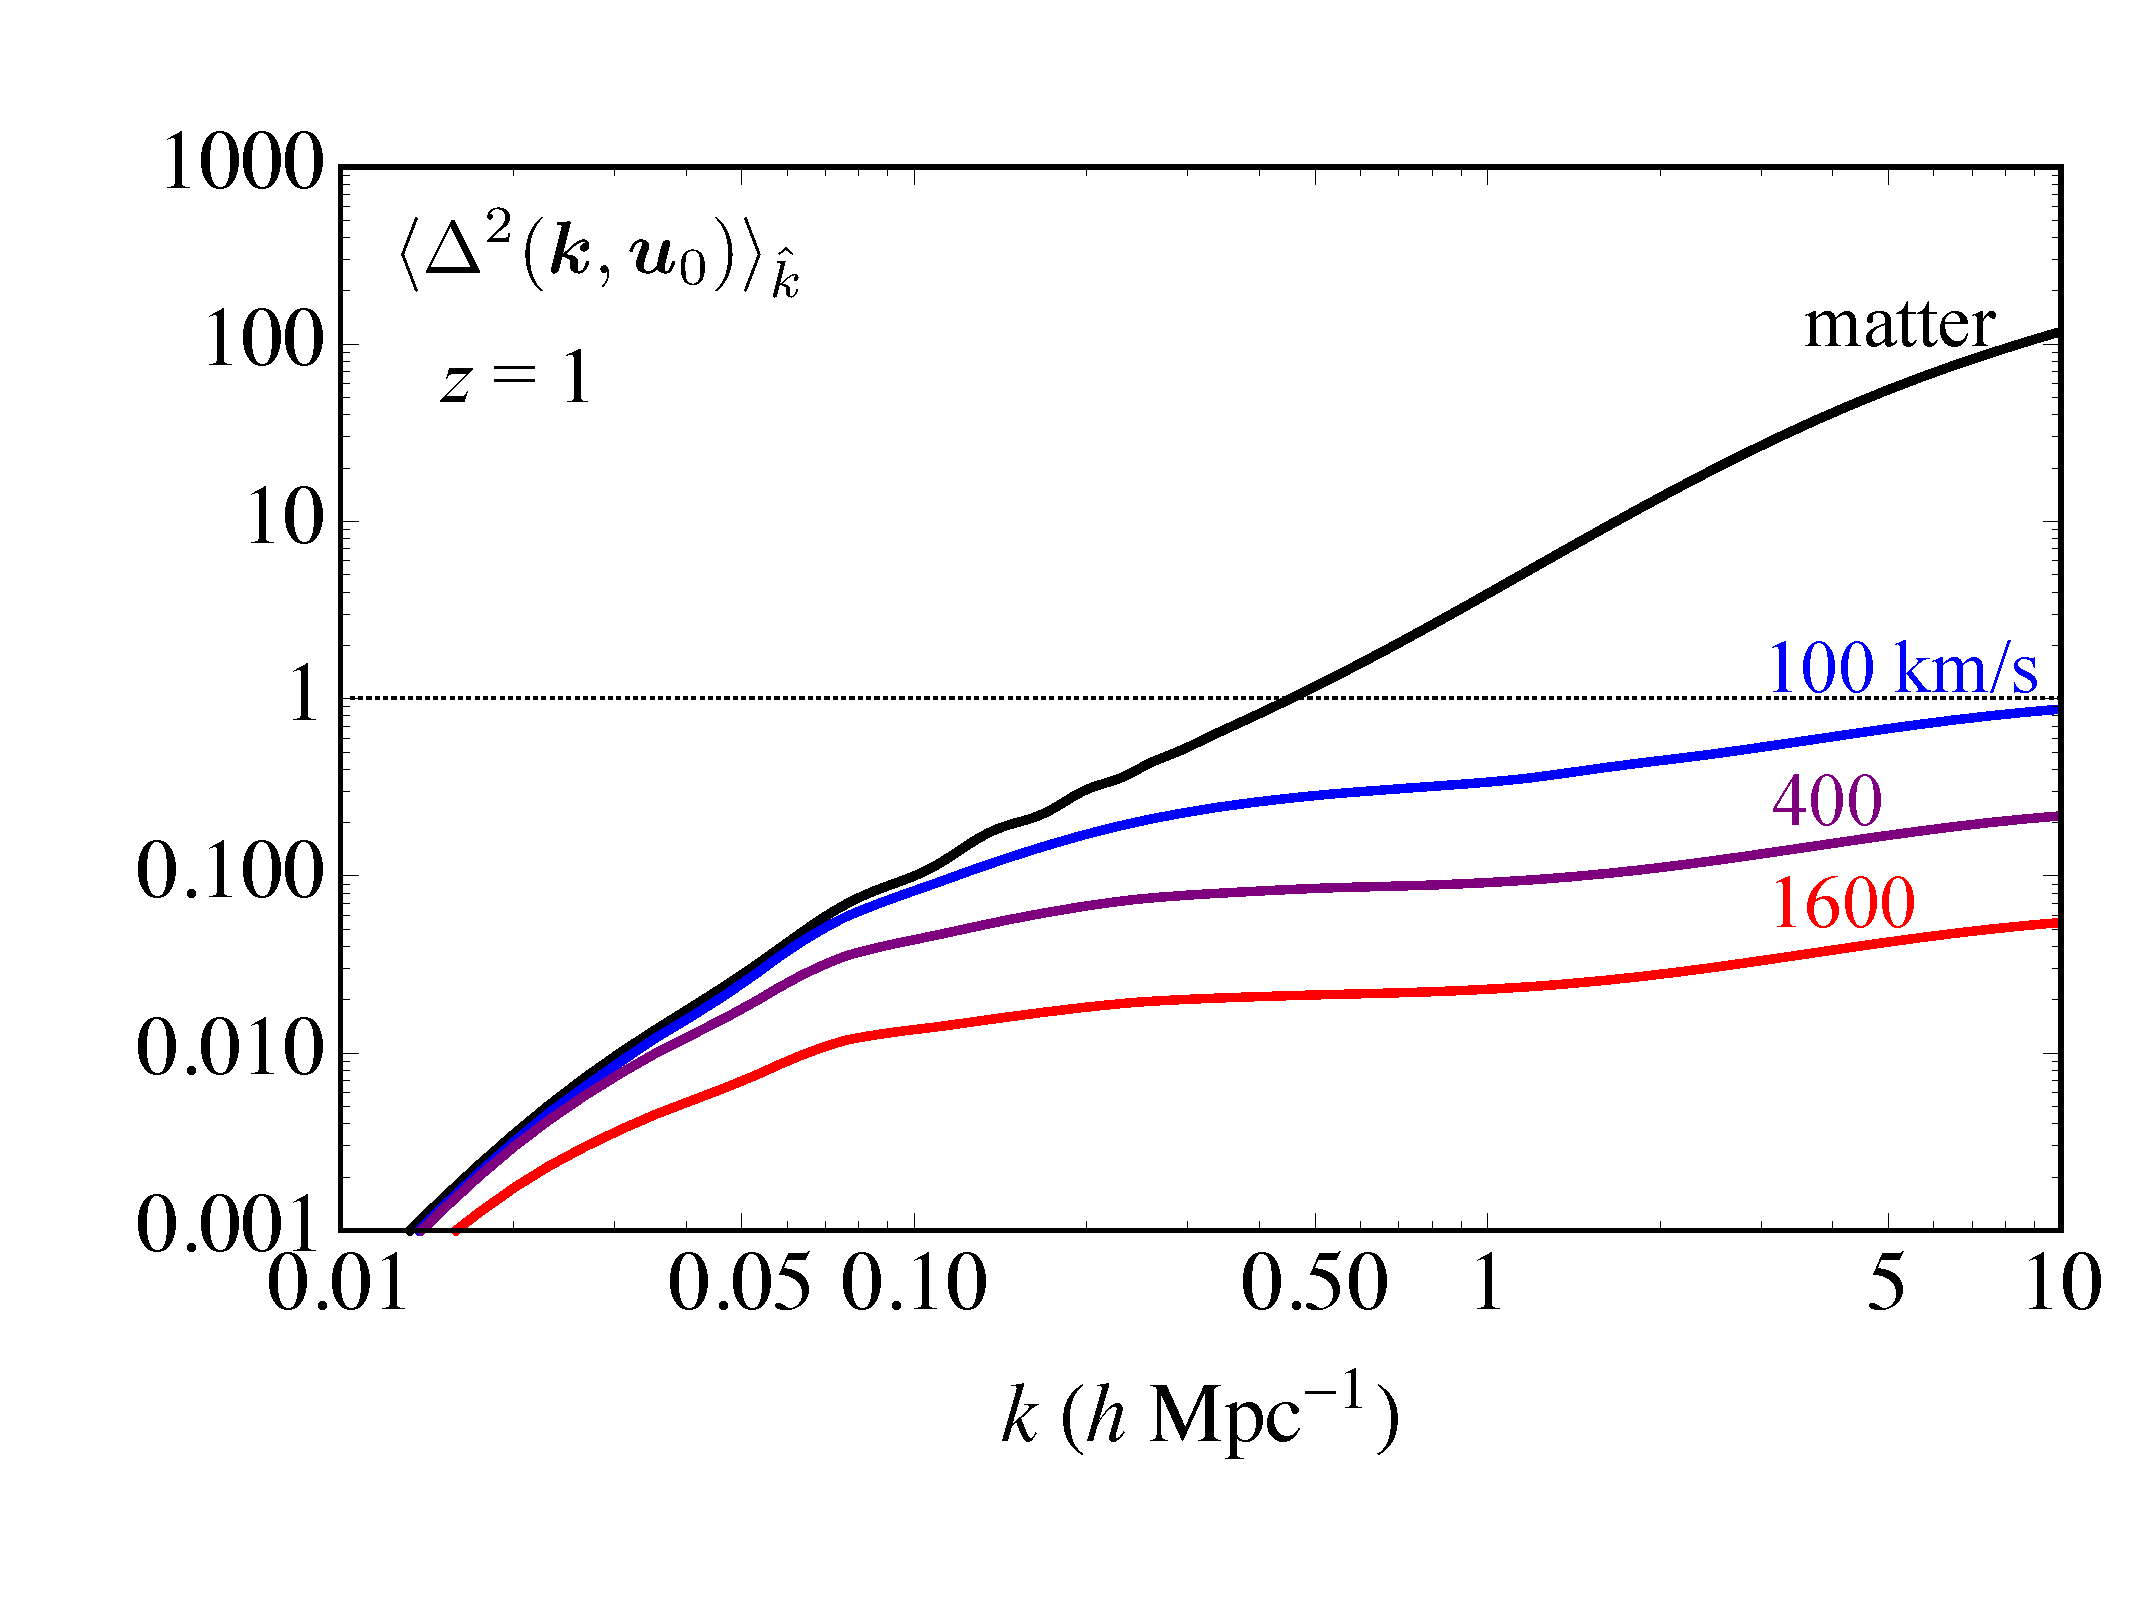
\includegraphics[width=0.47\textwidth]{nuplots/lin_resp_z1.pdf}
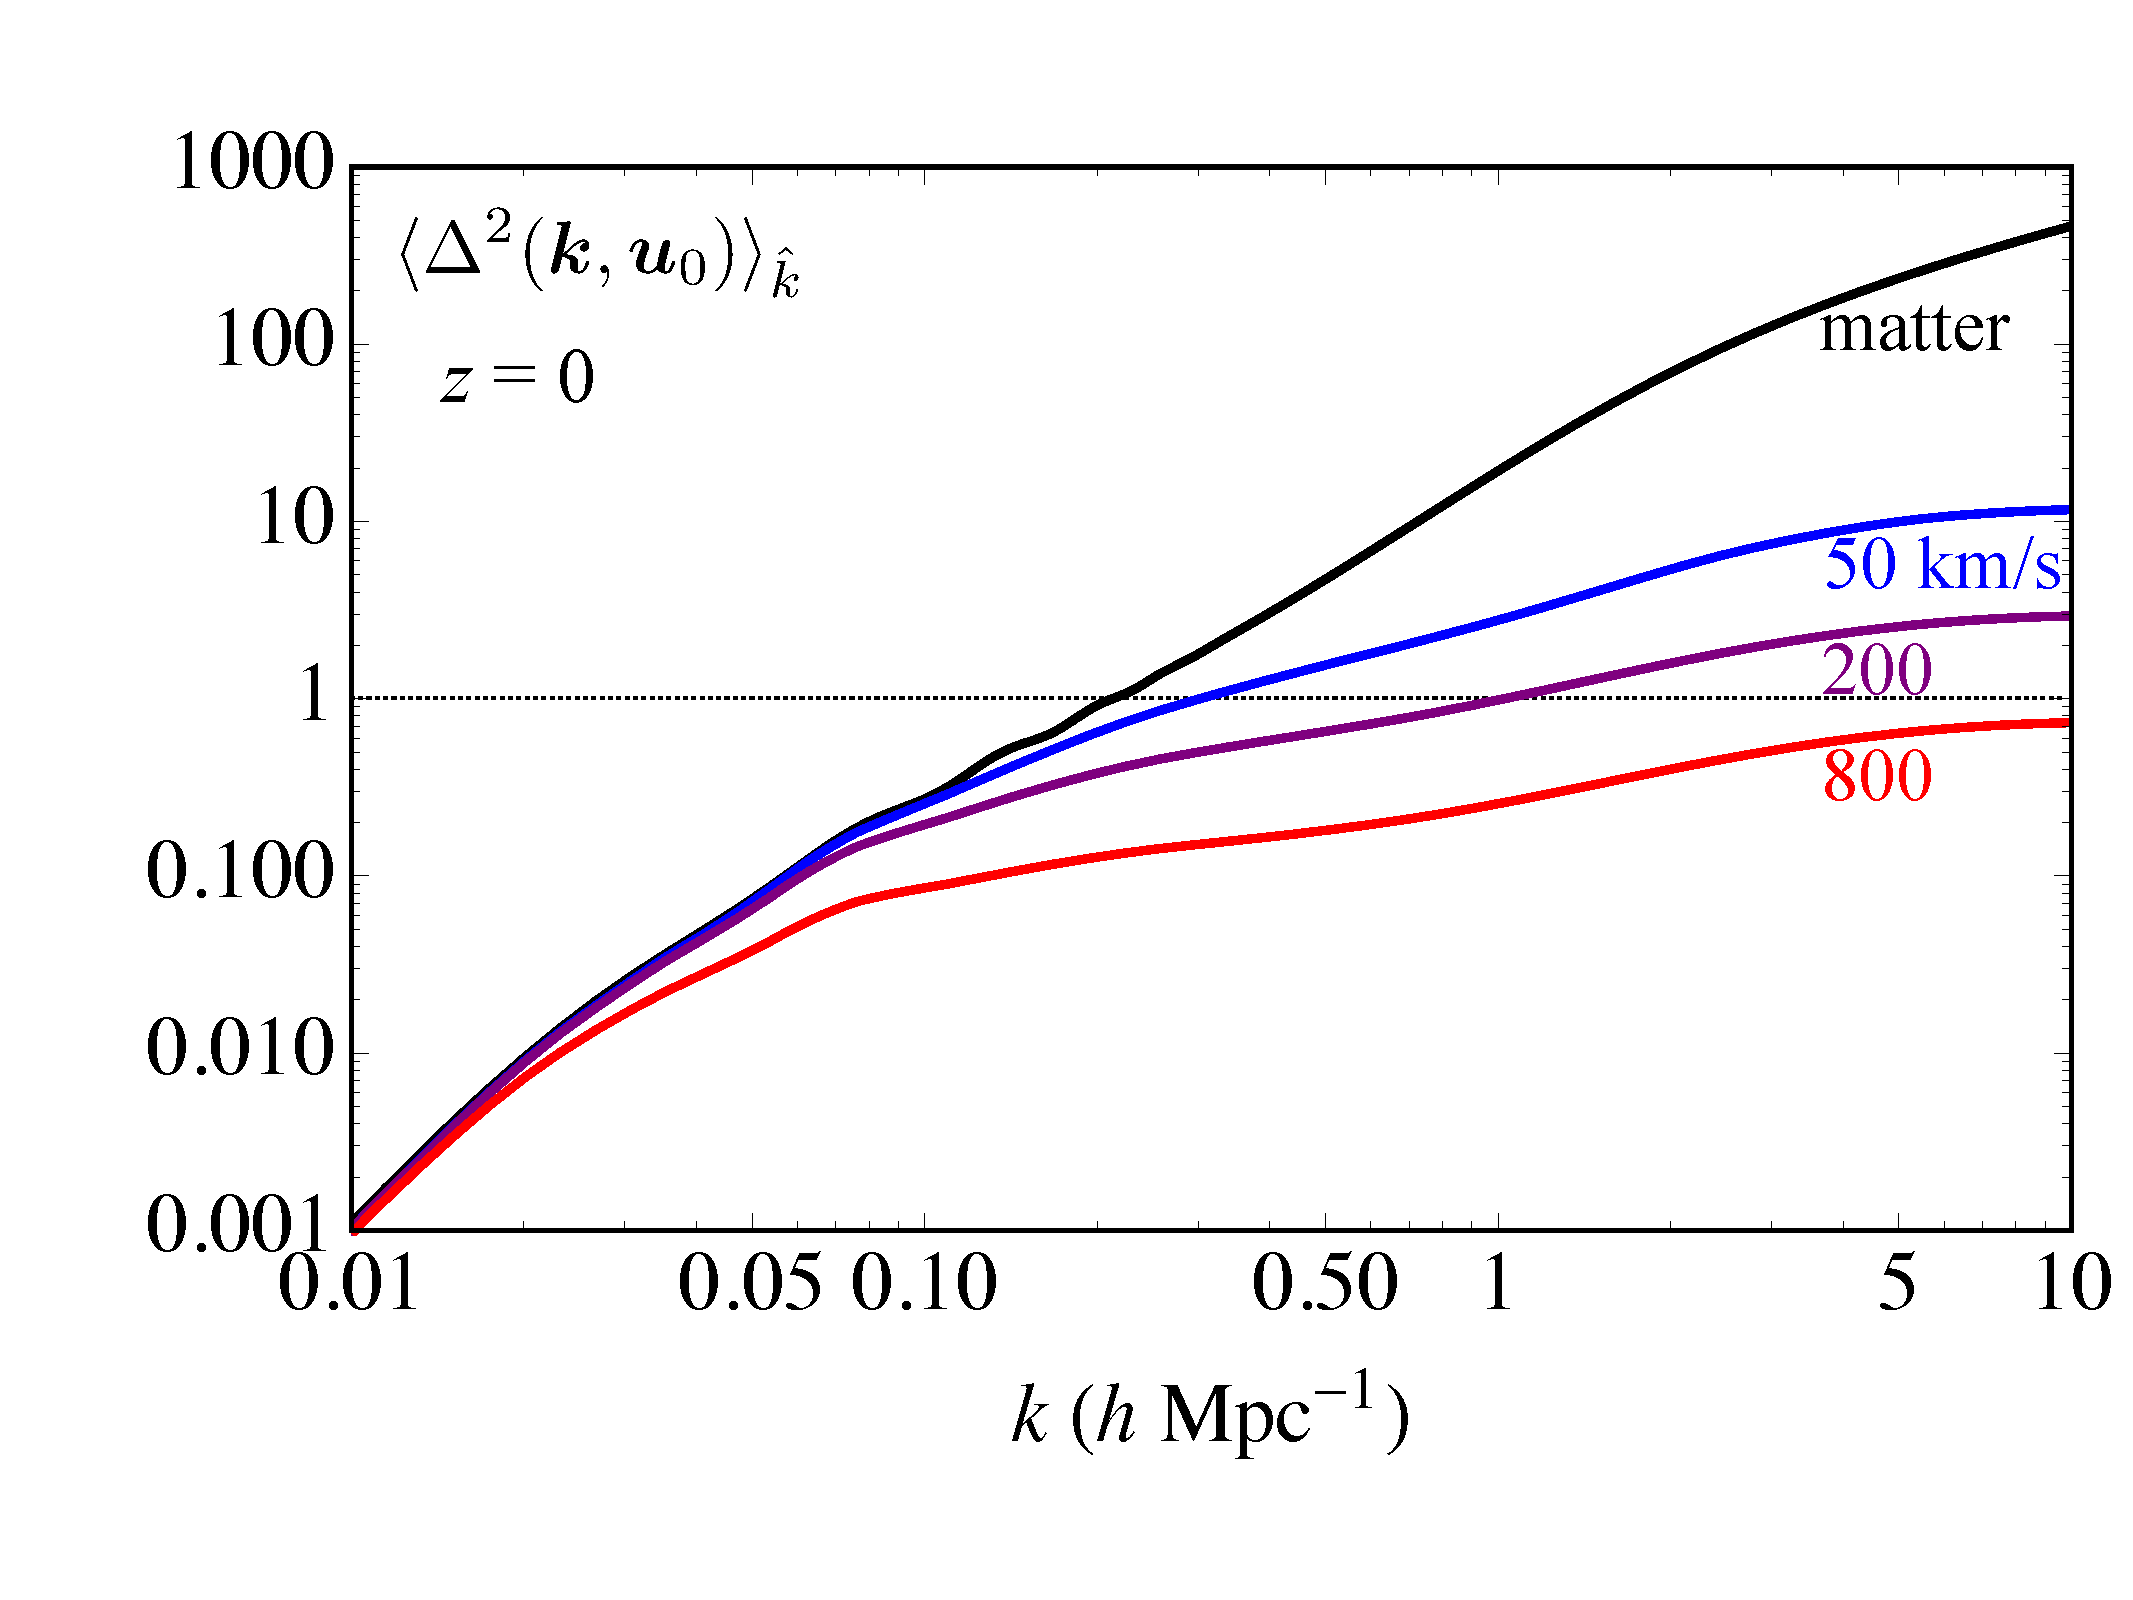
\includegraphics[width=0.47\textwidth]{nuplots/lin_resp_z0.pdf}
\caption{Angle-averaged power per logarithmic $k$-interval, in the linear-response approximation, for an unperturbed phase-space density $f^0(\bs{u}) = \delta_{\rm D}(\bs{u}- \bs{u}_0)$. The curves are labeled by the unperturbed velocity $u_0$. At redshift 1 (left panel), we see that particles with unperturbed velocities as low as $\sim 100$ km/s do not strongly cluster on all scales. At redshift 0 (right panel), particles with unperturbed velocities $u_0 \gtrsim 800$ km/s do not strongly cluster on all scales.}
\label{fig:halofitvshell}
\end{figure*}


\subsubsection{Single velocity shell}

%\spb{I think the main difference between this and 2.3 is the use of approximation \eqref{eq:phases}. But I did not realise this initially and may still be confused. I would like to unify the two sections as I do not like making the reader understand intermediate incorrect results, but we should discuss this in Pittsburgh.}

To confirm our estimates from the single velocity bin case, we now consider a single velocity \emph{shell}, so that we can compare our results to existing numerical results. We therefore consider the following isotropic unperturbed distribution, which is the average of the single-bin distribution over the direction of $\bs{u}_0$:
\beq
f^0_{u_0}(u) \equiv \langle f_{\bs{u}_0}^0 (\bs{u}) \rangle_{\hat{u}_0} = \frac1{4 \pi u_0^2} \delta_{\rm D}(u- u_0).
\eeq
In the LRA, the resulting overdensity is (neglecting the initial condition piece)
\barr
&&\delta_{u_0}(\bs{k}) = \langle \delta_{\bs{u}_0}(\bs{k}) \rangle_{\hat{u}_0} \nonumber\\
&&= \frac32 H_0^2 \Omega_M \int_{s_i}^s ds' (s - s') a' j_0[u_0 k (s - s')] \delta_{\rm M}(s', \bs{k}).~~~~~ \label{eq:delta-shell}
\earr
We denote the corresponding dimensionless power spectrum by $\Delta^2_{u_0}(k)$. Let us first point out that the inequality $|\delta_{\bs{u}_0} - \langle \delta_{\bs{u}_0}(\bs{k}) \rangle_{\hat{u}_0}|^2 \geq 0$ implies $\Delta^2_{u_0} \leq \langle \Delta^2_{\bs{u}_0} \rangle_{\hat{u}_0}$. Hence, imposing that $\langle \Delta^2_{\bs{u}_0} \rangle_{\hat{u}_0} \leq 1$ is a more stringent and relevant requirement than imposing $\Delta^2_{u_0} \leq 1$; in fact, we will see that the latter inequality can be amply satisfied even in regimes where the LRA fails.

Before computing the power spectrum, it is useful to simplify Eq.~\eqref{eq:delta-shell} further. In the linear regime, the matter overdensity is proportional to the direction-independent (but $k$-dependent) growth rate, so that
\beq
\delta_M(s', \bs{k}) \approx \left(\frac{P_M(s', k)}{P_M(s, k)}\right)^{1/2} \delta_M(s, \bs{k}). \label{eq:phases}
\eeq
On scales smaller than the free-streaming scale, the rapidly oscillating spherical Bessel function selects mostly times $s' \approx s$ in the integral of Eq.~\eqref{eq:delta-shell}. Hence, once again, provided $k_{\rm fs} \lesssim k_{\rm nl}$, the approximation Eq.~\eqref{eq:phases} leads to an accurate $\delta_{u_0}$ on all scales. While we made a similar argument to compute $\langle \Delta^2_{\bs{u}_0} \rangle_{\hat{u}_0}$ earlier, we stress that here, the argument applies to the overdensity field itself, rather than its power spectrum.

Inserting the approximation \eqref{eq:phases} into Eq.~\eqref{eq:delta-shell}, we find the power spectrum
\barr
\Delta^2_{u_0}(s, k)&\approx& \left(\frac32 \frac{H_0^2 \Omega_M}{k u_0}\right)^2\nonumber\\
&\times& \left[\int_{s_i}^s ds' a' \sin[k u_0 (s - s')] \Delta_M(s', k) \right]^2. ~~~~~
\earr
We compare this approximation with the shot-noise-reduced $N$-body simulations of \cite{Banerjee_2018}, hereafter B18. In this work, massive neutrinos were simulated with the $N$-body method, but with optimized initial conditions in order to reduce shot noise: instead of assigning neutrinos with a random velocity direction at each grid point, $12 ~N_{\rm side}^2$ particles are assigned to each grid point, with an isotropic velocity distribution using the \textsc{healpix} algorithm \citep{Healpix}. Specifically, we compare to the simulation \texttt{LU\_SH10\_NS2} of B18, for which $48 \times 128^3$ neutrino particles were used per velocity shell, for 10 shells ranging from 495 km/s to 5773 km/s, corresponding to a total of approximately $1000^3$ neutrino particles.

The comparison with B18 is shown in Fig.~\ref{fig:simvshell}. On large enough scales, we find that the power spectra computed with both methods agree very well (up to sample-variance deviations on scales comparable to the box size of B18). For unperturbed velocities $u_0 \gtrsim 800$ km/s, the results of B18 show clear evidence of residual shot noise, and start deviating from ours at increasingly large scales as the velocity is increased. However, they agree very well with our results on all scales where shot noise is subdominant. Only for the smallest velocity shell considered in B18, $u_0 = 495$ km/s, do we find that our results under-estimate the non-linear clustering of neutrinos, by a factor no larger than 2, for scales $k \gtrsim 0.1~h$ Mpc$^{-1}$. This departure occurs despite the fact that $\Delta^2_{u_0}$ is at most $\sim 0.05$, which again emphasizes that the perturbation of a velocity shell is not a good indicator of the validity of the LRA.
%\spb{My initial reading of this segment was that it implies that the comparison to Banerjee results is not convincing, because it uses this isotropic shell formalism, which we show to be inaccurate later. We should re-word this so that is less confusing!}
The excellent agreement of our results with their numerical counterparts corroborates our previous finding that the LRA is accurate for $u_0 \gtrsim 800$ km/s at $z = 0$. Since the free-streaming scale corresponding to $u_0 \gtrsim 800$ km/s is well in the linear regime, we are justified a posteriori in using Eq.~\eqref{eq:phases}. We will check explicitly later on that neutrinos with $u_0 \gtrsim 800$ km/s are very well correlated with the matter field, as is implied by this approximation.


\begin{figure}
  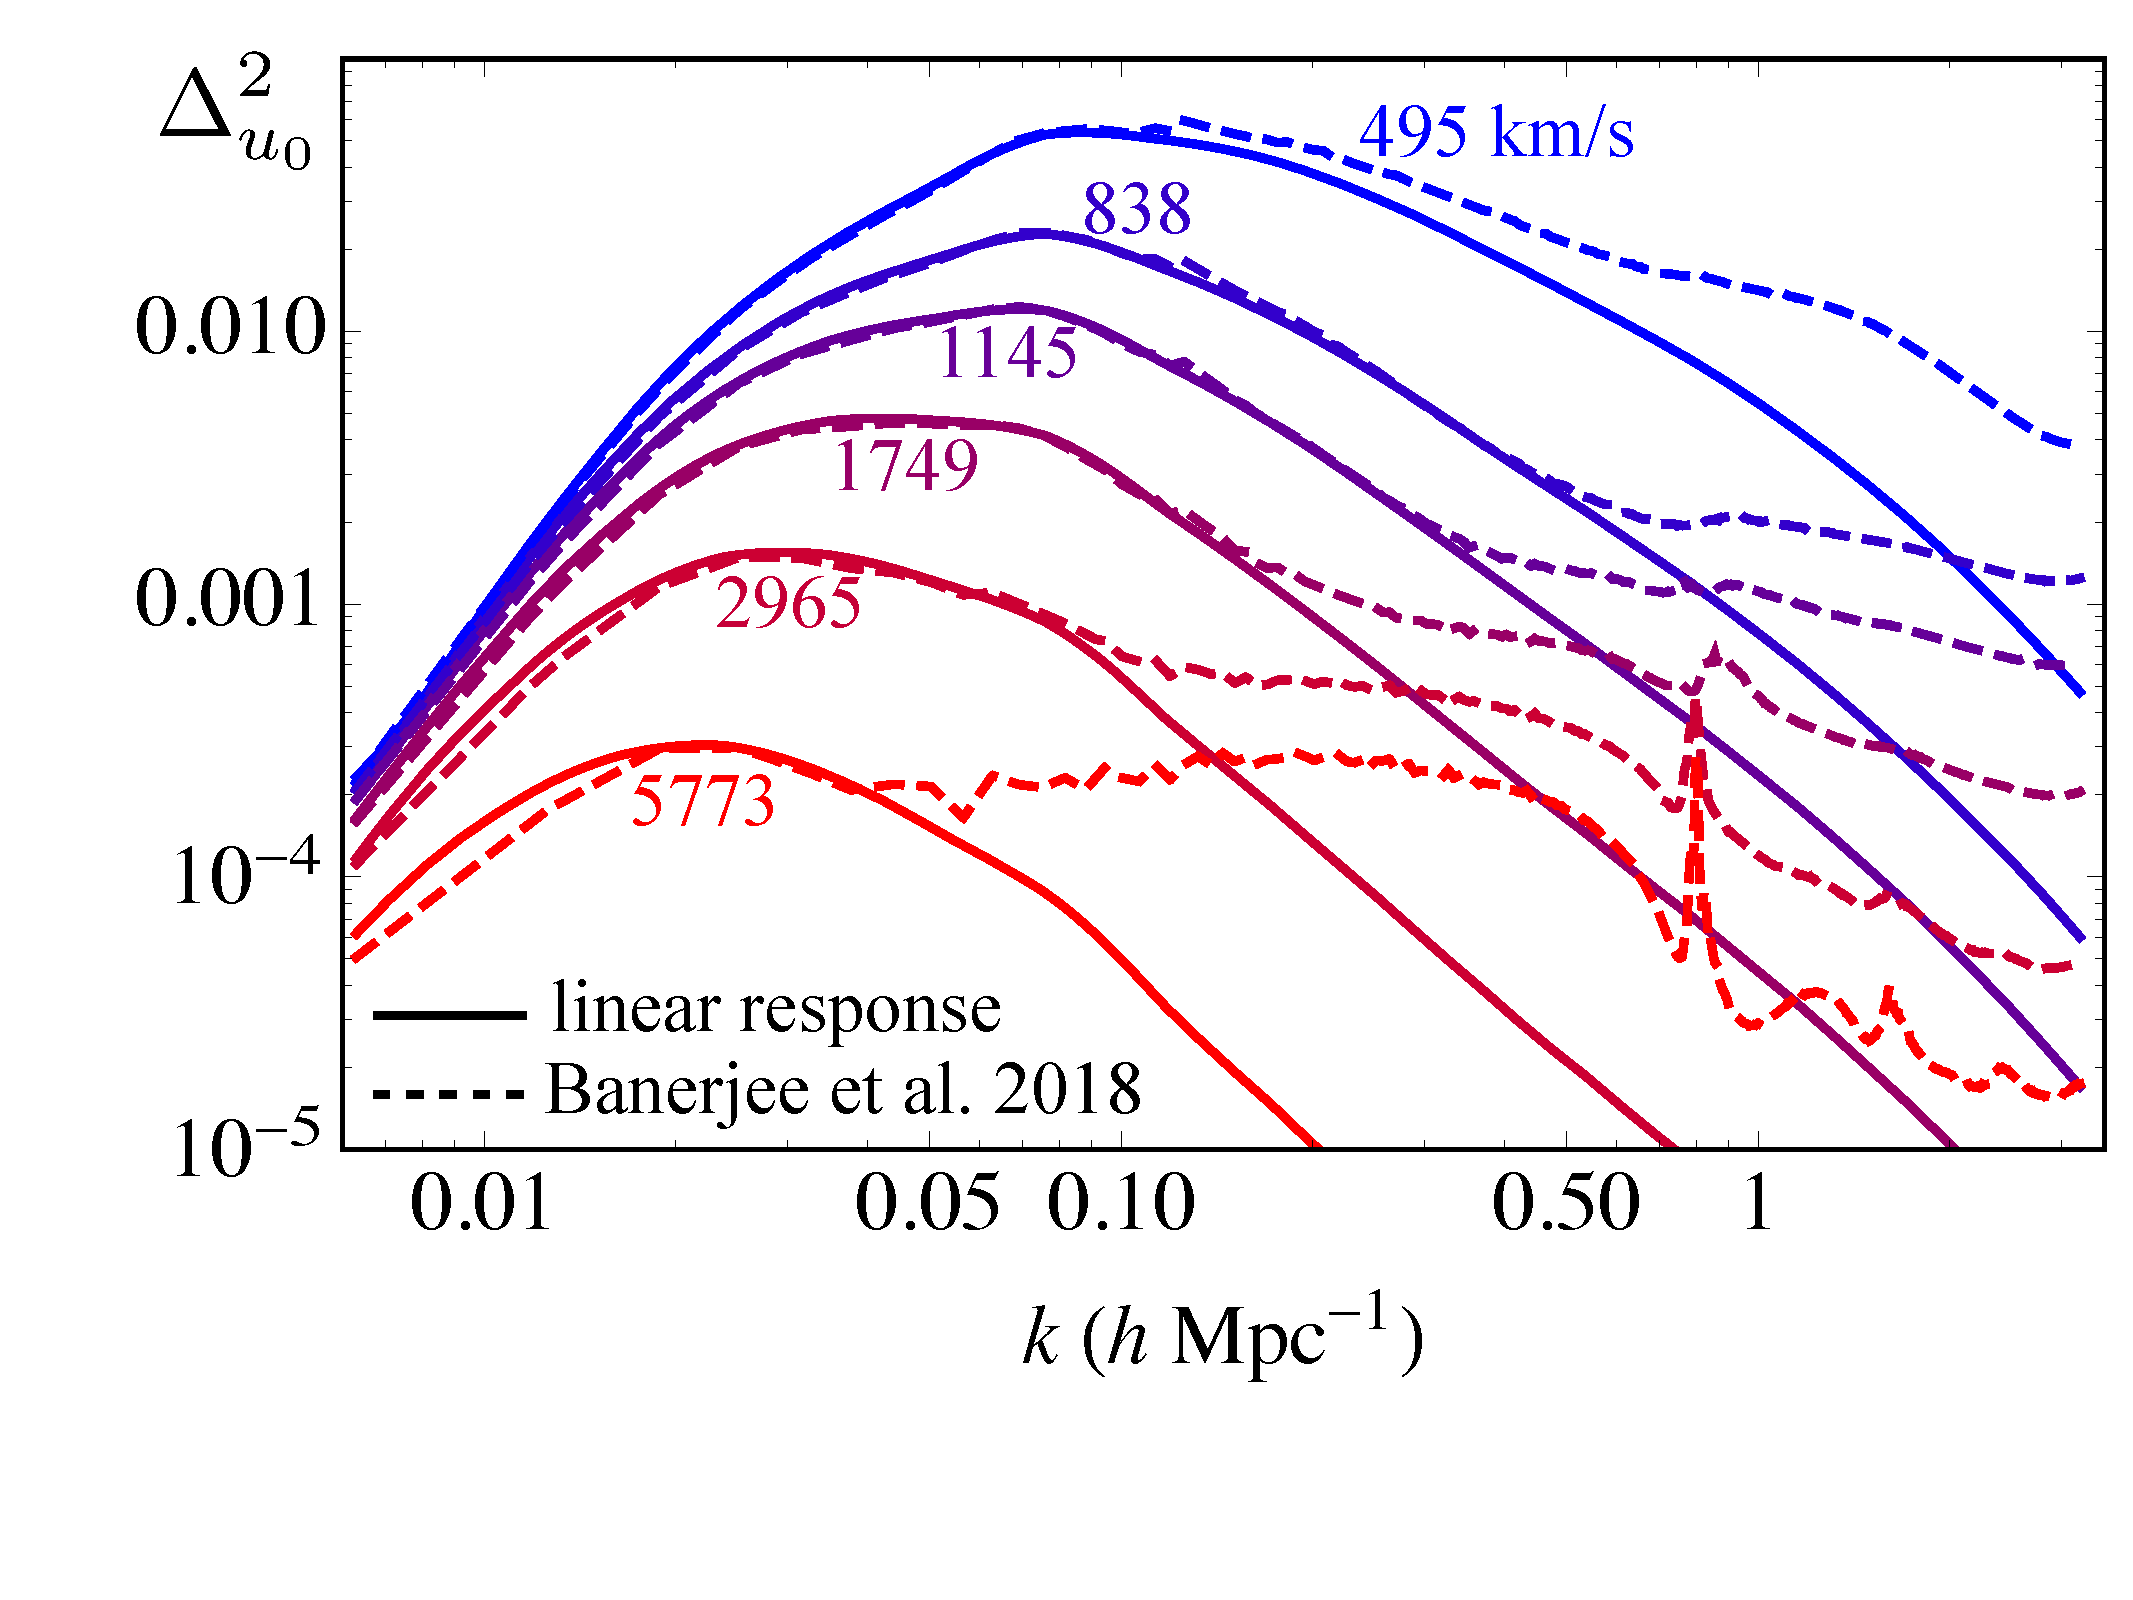
\includegraphics[width=0.45\textwidth]{nuplots/banerjee_lin_resp.pdf}
  \caption{Power per logarithmic $k$-interval in different velocity shells at $z = 0$, in the linear-response approximation (LRA, solid), and from the simulations of \protect \cite{Banerjee_2018} (dashed). The agreement is excellent for $u_0 \gtrsim 800$ km/s, except for departures at small scales clearly due to residual shot noise in the particle simulations. Only for the lowest velocity shell shown does the LRA noticeably underestimate clustering.
  %\spb{I would like to include both plots: this one shows us that the particles and analytics match up to 800 km/s. The other shows us that we would expect them to match, because we are in a regime where perturbation theory works.}
  }
  \label{fig:simvshell}
\end{figure}


\subsection{Application to fast massive neutrinos}

Having established the regime of validity of the LRA, we may now apply it to arbitrary phase-space densities, provided they are restircted to velocities $u \geq v_{\rm crit}$. In addition, since in the regime of validity of the LRA, the free-streaming scale is larger than the non-linear scale, we may also safely make the approximation \eqref{eq:phases} in the integral \eqref{eq:delta-phi}.

Let us apply the LRA to a truncated Fermi-Dirac distribution, which describes the unperturbed velocity distribution of neutrinos faster than $v_{\rm crit}$:
%Once the slow neutrinos are followed as particles, the LRA is applied only to ``fast'' neutrinos, that is, the portion of the neutrino phase space with unperturbed velocities higher than the cutoff velocity.
%The unperturbed density of these particles is given by the truncated Fermi-Dirac distribution:
\begin{equation}
f^0(u) \propto \Theta(u - v_{\rm crit}) \left(\rme^{m_\nu u/ \left(k_\mathrm{B} T_\nu\right)} + 1 \right)^{-1},
\end{equation}
where $\Theta$ is the Heaviside function (or an infinitesimally smoothed version of it, so that $f^0$ is differentiable), $m_\nu$ is the mass of a single neutrino or antineutrino, $k_\mathrm{B}$ is the Boltzmann constant in eV/K and $T_\nu \approx 1.97$ K is the temperature of the cosmic neutrino background. The normalization is again such that $\int d^3 u f^0(u) = 1$. The kernel in Eq.~\eqref{eq:delta-phi} is therefore given by
\barr
\mathcal{I}(\kappa) = \frac{\int_{q_c}^{\infty} dq~ j_0\left(\kappa \frac{T_\nu}{m_\nu}q\right)~ q^2 /(\rme^q + 1) }{\int_{q_c}^{\infty} dq ~q^2/(\rme^q + 1)}, \ \ \ q_c \equiv \frac{m_\nu v_{\rm crit}}{T_\nu}.
\earr
We use the following asymptotic expansion for the integral:
\begin{align}
 \int^\infty_{q_\mathrm{c}} \frac{j_0(qX)}{e^q + 1} q^2 dq &= - \sum^{\infty}_{n=1} (-1)^n \frac{\rme^{-n q_\mathrm{c}}}{(n^2+X^2)^2} I_n(q_\mathrm{c},X),\\
 I_n(q_\mathrm{c},X) &= \left(n^2 + n^3 q_\mathrm{c} + n q_\mathrm{c} X^2 - X^2\right) \frac{\sin(q_\mathrm{c} X)}{X} \nonumber \\
 &+ \left(2n + n^2 q_\mathrm{c} + q_\mathrm{c} X^2\right) \cos(q_\mathrm{c} X),
\end{align}
We have checked that this expansion is converged to within an absolute error of $< 10^{-4}$ for $n_\mathrm{max} = 20$. We show the kernel $\mathcal{I}$ for different values of $v_{\rm crit}$ in Fig.~\ref{fig:kernel}.

\begin{figure}
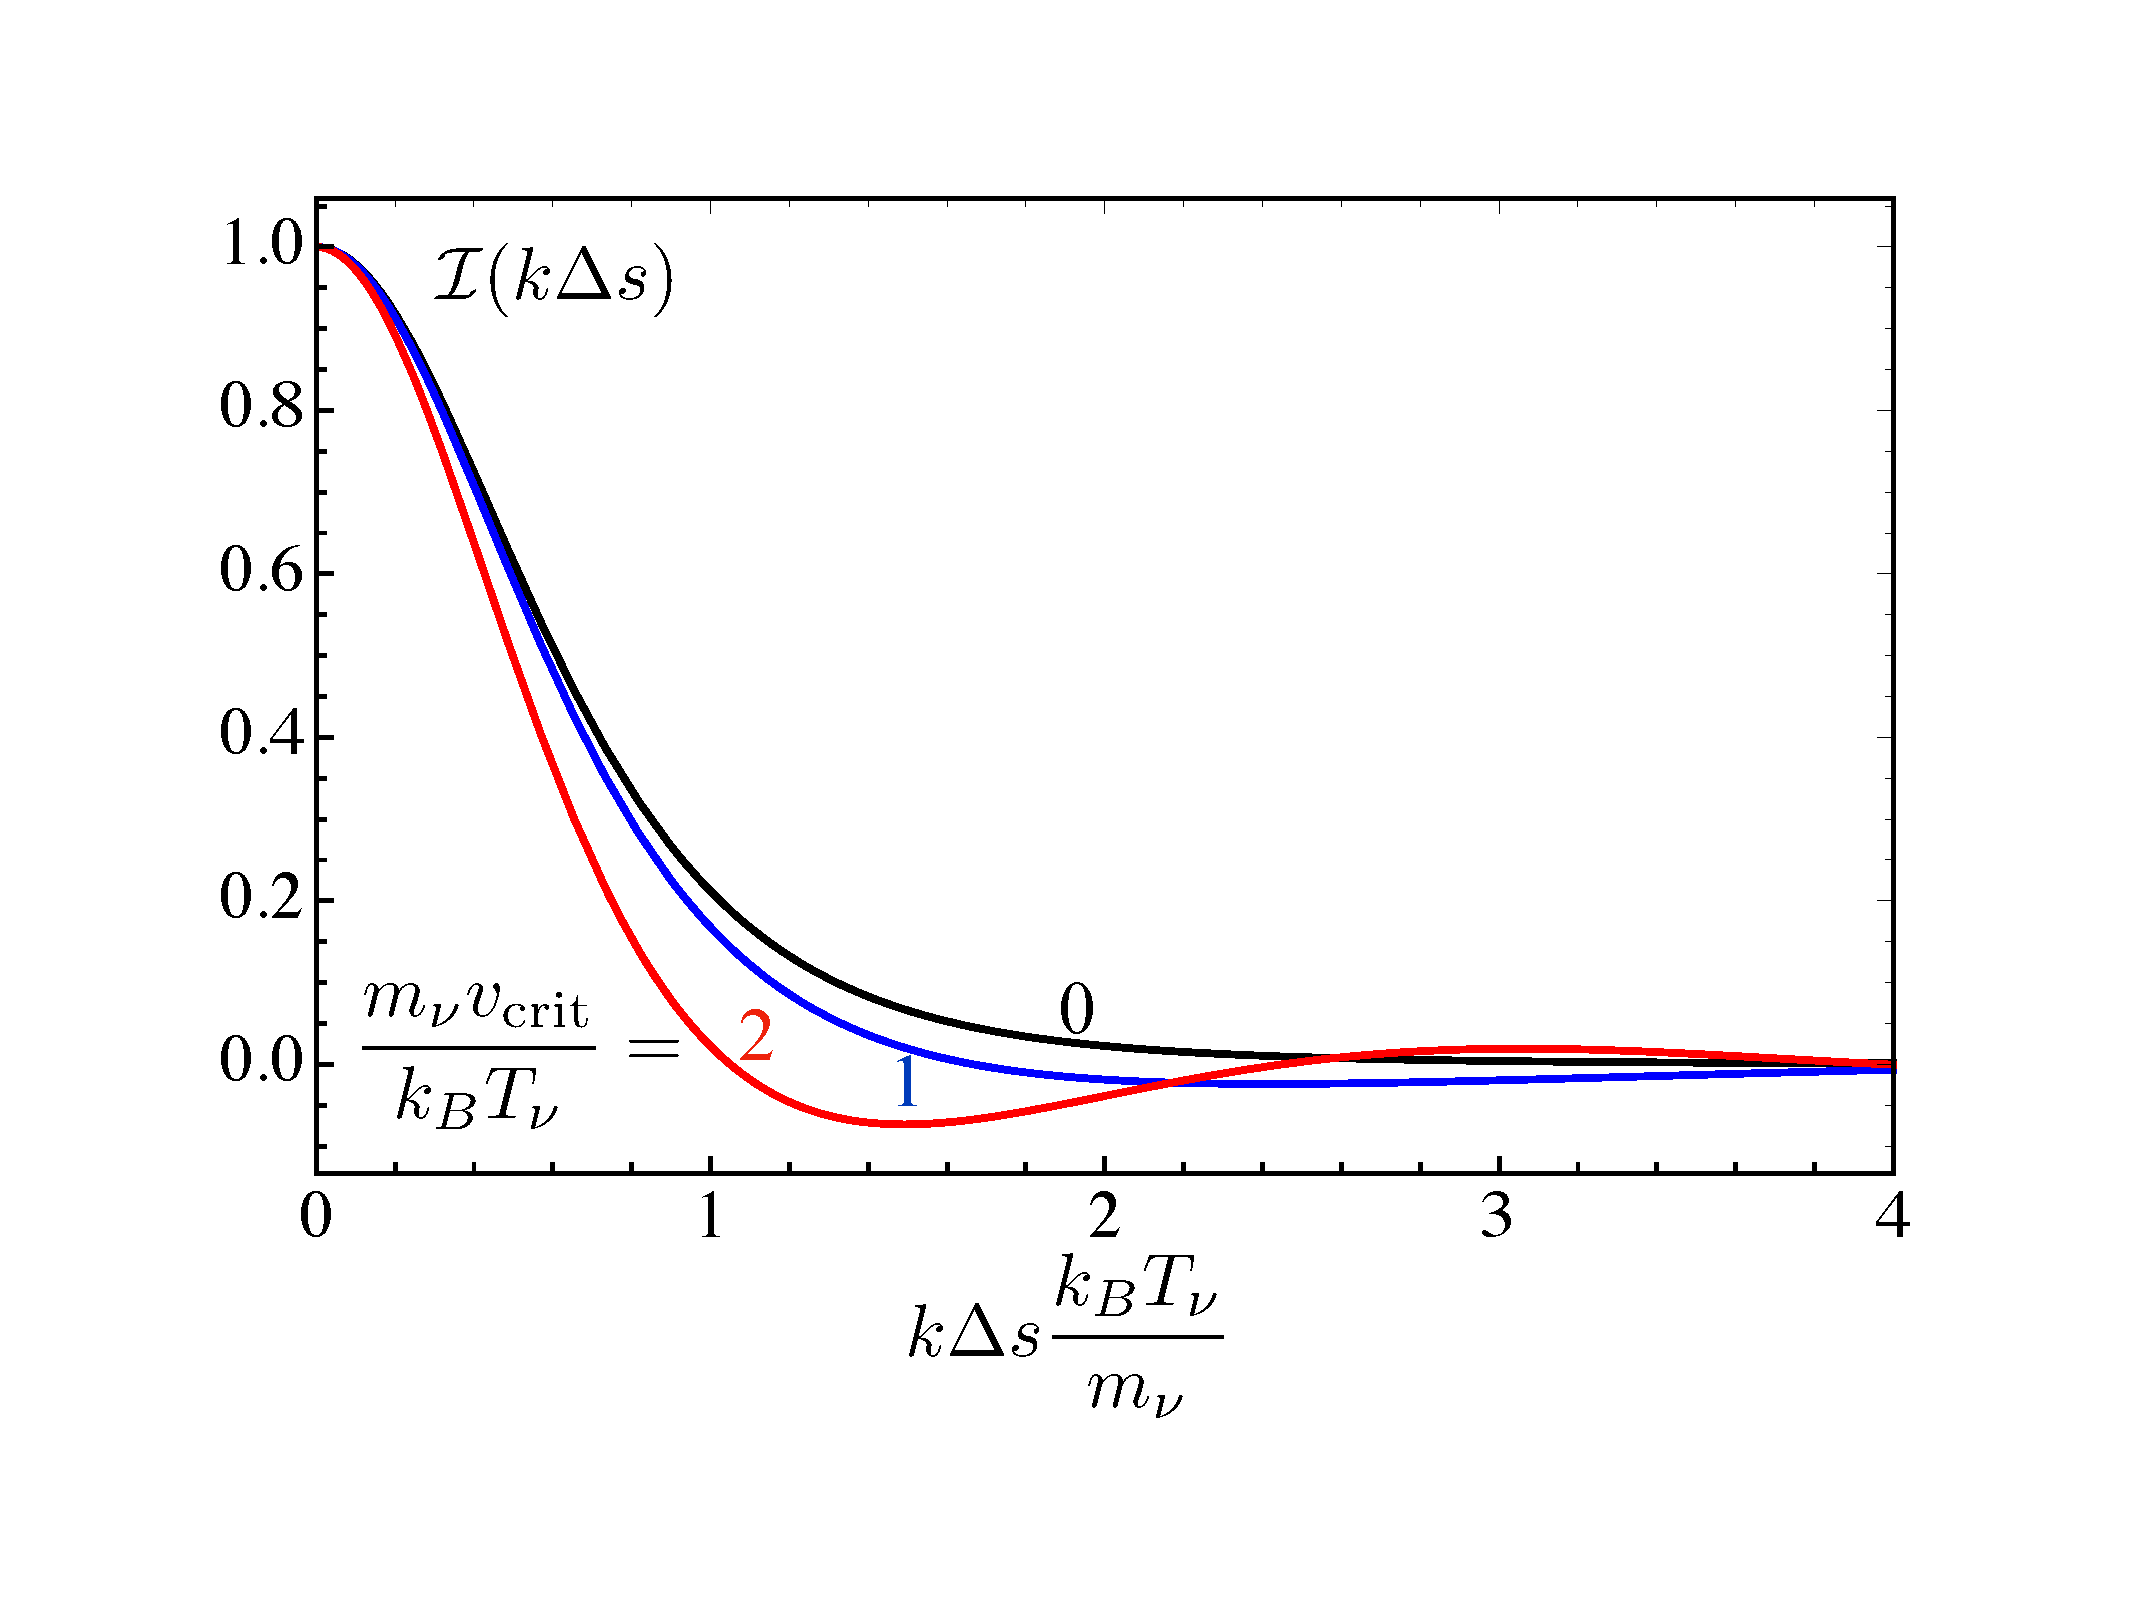
\includegraphics[width=0.43\textwidth]{nuplots/kernel.pdf}
%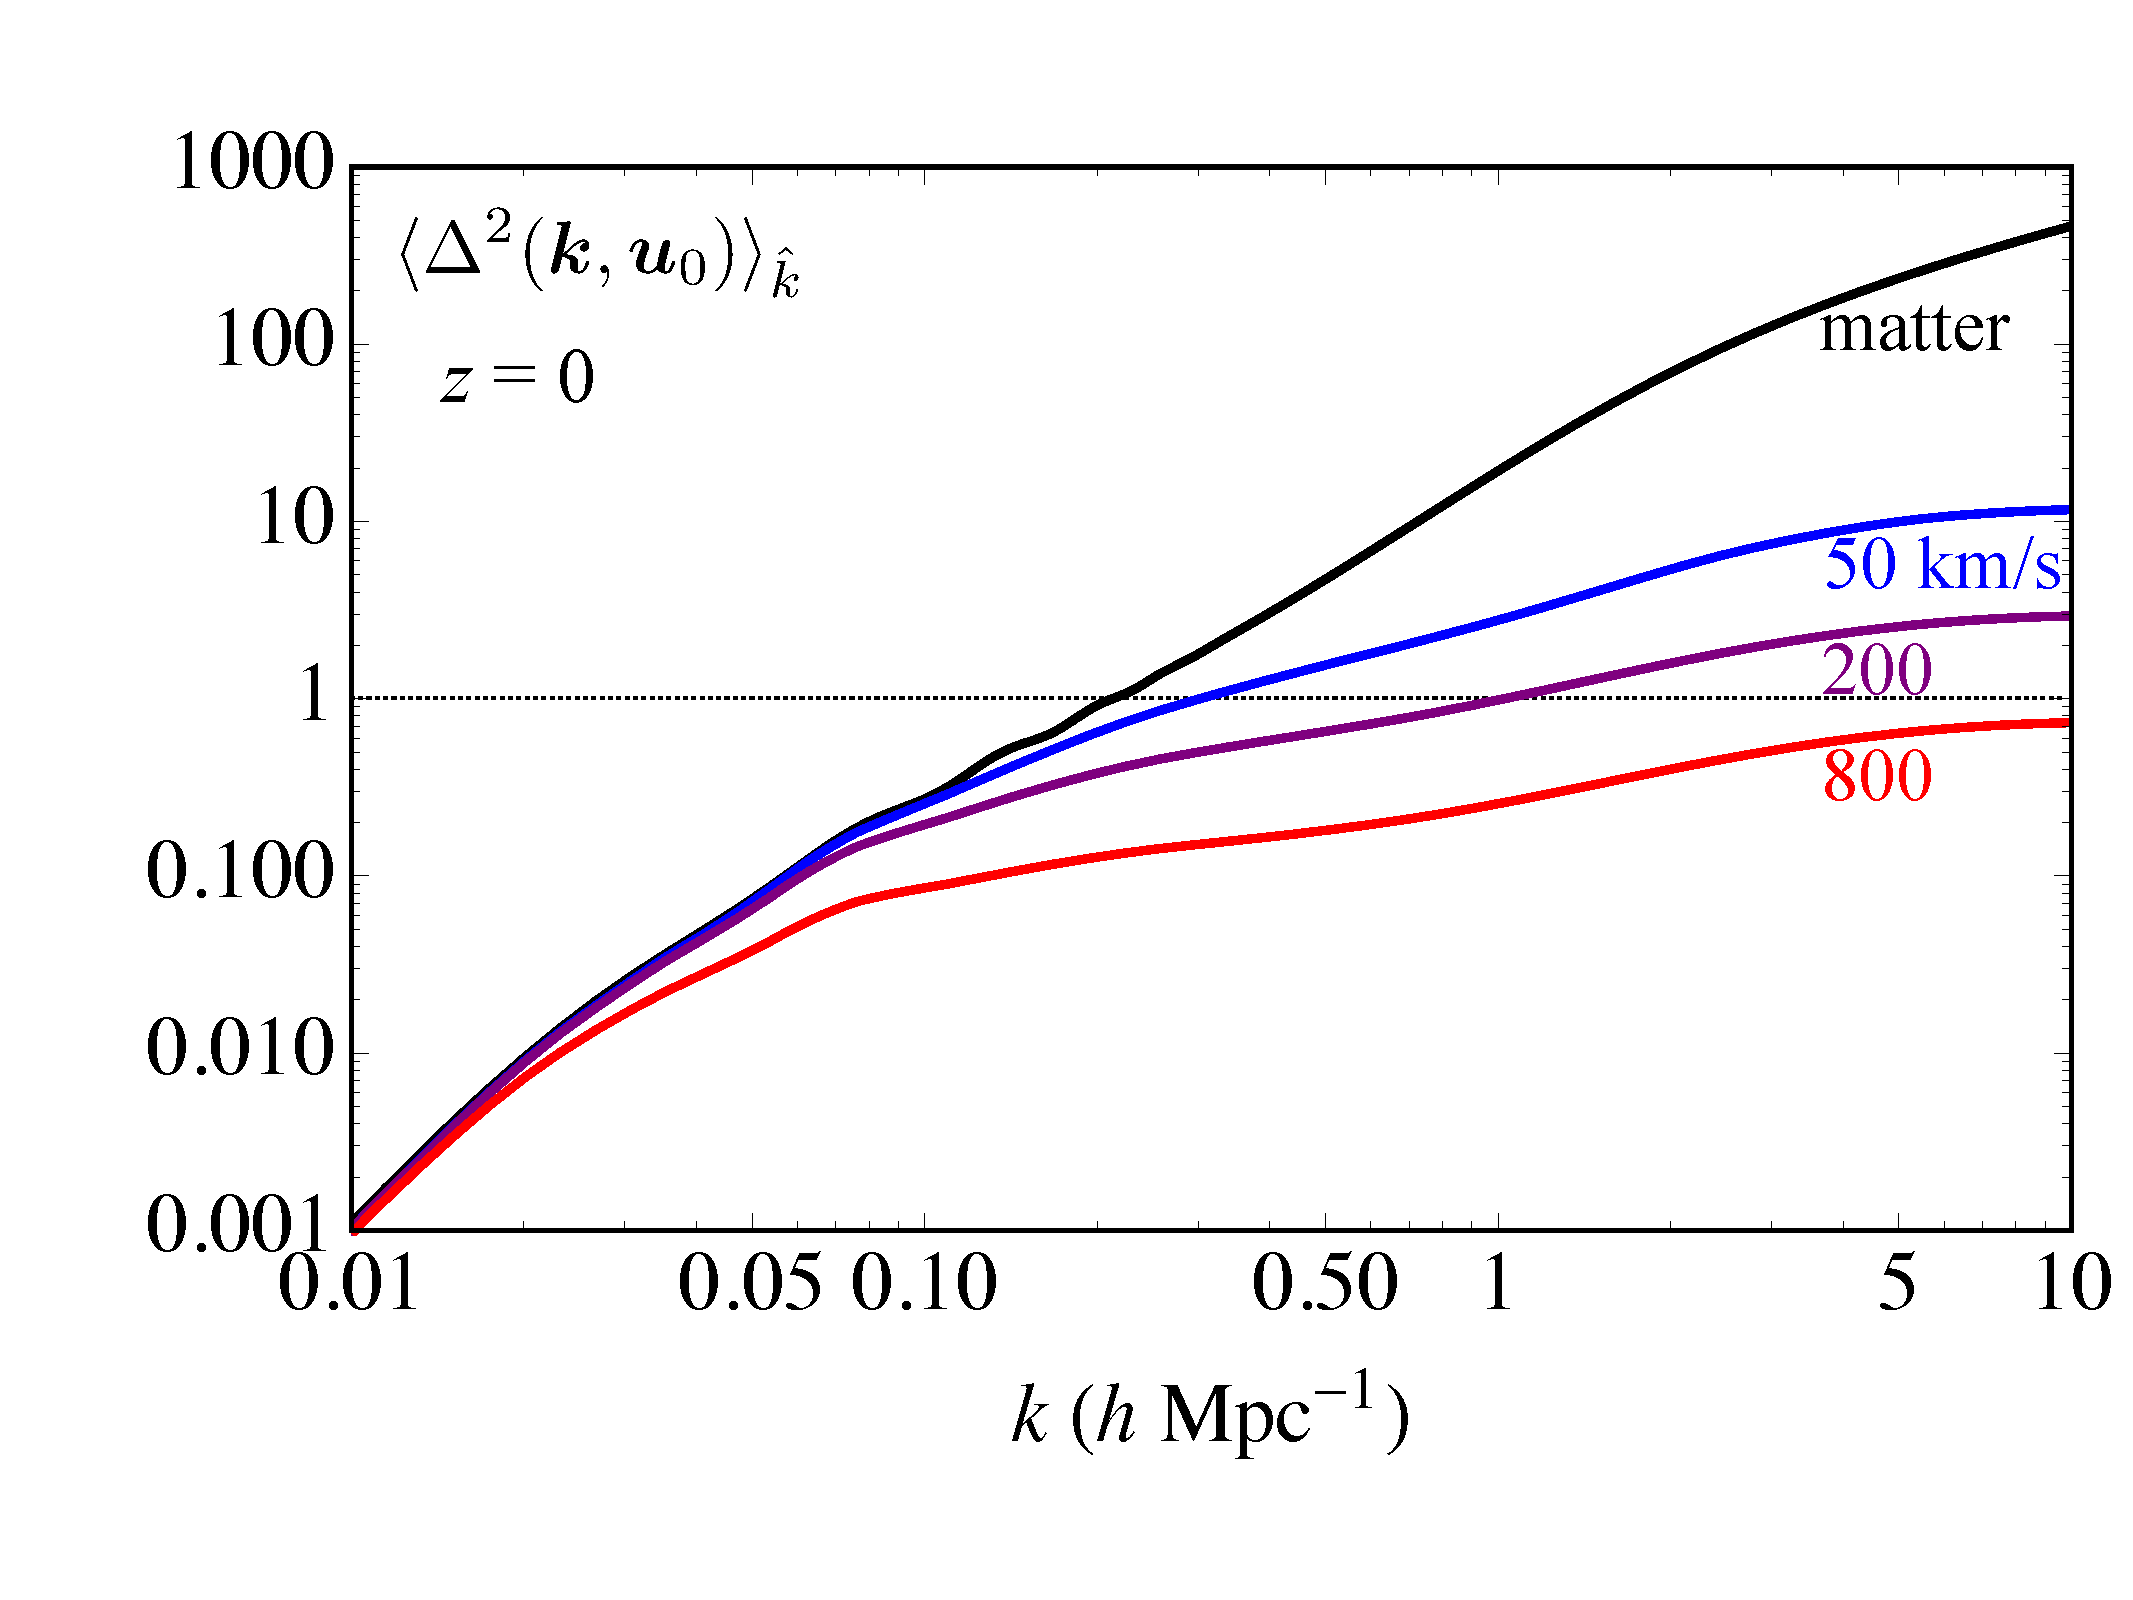
\includegraphics[width=0.47\textwidth]{nuplots/lin_resp_z0.pdf}
\caption{Kernel $\mathcal{I}(k \Delta s)$ defined in Eqs.~\eqref{eq:delta-phi}, \eqref{eq:I(k)} for a truncated Fermi-Dirac distribution restricted to $u \geq v_{\rm crit}$, for several values of $m_\nu v_{\rm crit}/T_\nu$. }
\label{fig:kernel}
\end{figure}


\section{Hybrid method} \label{sec:hybrid}

\subsection{Basic idea and default parameters}

The basic idea of the hybrid method we propose is to split neutrinos into a ``slow" and a ``fast" component, depending on their \emph{unperturbed} velocity relative to some critical velocity $v_{\rm crit}$, as illustrated in Fig.~\ref{fig:fddistribution}. We emphasize that this split is performed in the unperturbed velocity; acceleration due to passing in and out of potential wells formed by structure may cause ``slow'' particles to acquire a large perturbed velocity, and ``fast'' particles to slow down. The ``slow" and ``fast" labels can be thought of ``Lagrangian'' labels, which allow both the slow and fast components to independently satisfy the collisionless Boltzmann equation\footnote{If the split between ``slow" and ``fast" had been made instead in terms of the perturbed or ``Eulerian" velocity, one would have to solve for two coupled collisional Boltzmann equations to account for the flux of particles across the boundary.}. We are free to solve these two equations with different techniques: the LRA for fast particles and the $N$-body method for slow particles. This allows us to focus the computationally expensive $N$-body technique on the fraction of phase-space where it is truly needed.

\begin{figure}
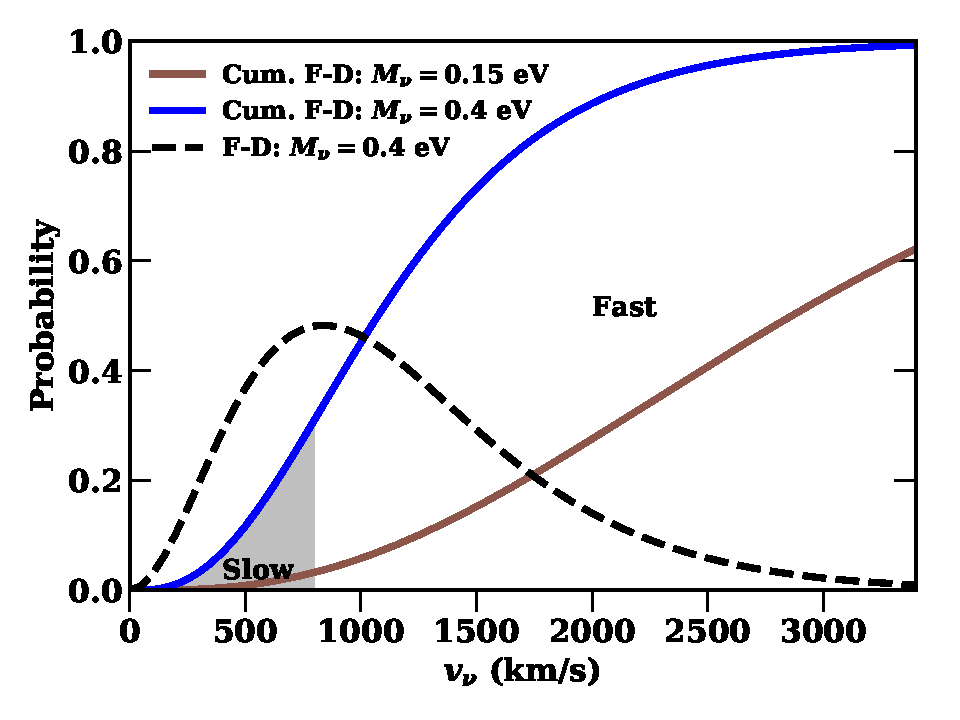
\includegraphics[width=0.45\textwidth]{nuplots/fermidirac.pdf}
  \caption{The integrated Fermi-Dirac distribution, showing the cumulative probability for neutrinos to have an unperturbed velocity less than $v_\nu$ at $z=0$ for total neutrino mass $M_\nu = 0.4$ eV.
  The grey shaded region shows the neutrino density followed by particles in our hybrid method.
  }
  \label{fig:fddistribution}
\end{figure}

We could in principle set a time-dependent velocity boundary $v_{\rm crit}(z)$. However, this would require constantly converting fast particles into slow particles, since the range of validity of the LRA decreases with time, as neutrinos redshift and gravitational potentials deepen. Instead, we use the LRA for \emph{all} neutrinos down to a redshift $z_\nu$, after which we use a fixed $v_{\rm crit}$ down to $z = 0$. Our hybrid method thus has two adjustable parameters, $z_\nu$ and $v_{\rm crit}$. The choice of $z_\nu$ must be such that the fraction of neutrinos that are not accurately described by the LRA at $z \geq z_\nu$ is sufficiently small that it has no significant impact on any observables. The choice of $v_{\rm crit}$ must be such that neutrinos with $u_0 \geq v_{\rm crit}$ are accurately described by the LRA all the way to the present time.

We saw in Section \ref{sec:single-bin} that we expect the LRA to be accurate for $u_0 \gtrsim 100$ km/s at $z \geq 1$. For a relativistic Fermi-Dirac distribution with temperature $T_\nu = 1.95$ K, the fraction of neutrinos with unperturbed velocity less than $100$ km/s is
\beq
P(u < 100 ~\textrm{km/s}) \approx 6.7 \times 10^{-4} \left(\frac{m_{\nu}}{0.1~\textrm{eV}}\right)^3.
\eeq
Therefore, by treating \emph{all} neutrinos with the linear-response approximation at $z \geq 1$, we underestimate the clustering of at most $\sim 0.1\%$ of the neutrinos, given current upper bounds to their masses.
Even if these slow neutrinos cluster as strongly as the CDM (a substantial over-estimate), they cannot affect the total matter power on any scale. The maximum fractional error on $P_\mathrm{m}(k)$ is bounded by $\sim 10^{-3} \times 10 f_{\nu}$, where $f_\nu \approx 0.02 (M_\nu/0.3 \textrm{eV})$ is the fraction of matter in neutrinos, and the factor of $10$ accounts for the cumulative linear theory effect of neutrinos.
We see that this error should be very small, so we deem it safe to use the method of AHB13 (the LRA applied to \emph{all} neutrinos) for $z \geq 1$, i.e.~to set $z_\nu = 1$.\footnote{Note that the particle based method of \cite{Banerjee_2018} does not resolve neutrino velocities below several hundred km/s at all in their default setup, even for neutrino masses as low as $M_\nu = 0.15$ eV).}

We also saw in Section \ref{sec:validity} that the LRA is accurate at $z = 0$ for $u_0 \gtrsim 800$ km/s. To be conservative, we use a default neutrino critical velocity of $850$ km/s for $0 \leq z \leq z_\nu$. For reference, the fraction of slow neutrinos is $P(u < 850 ~\textrm{km/s}) \approx [0.04, 0.20, 0.42]$, respectively, for  $m_{\nu} = [0.05, 0.1, 0.15]$ eV.

In addition to the LRA, we use the approximation \eqref{eq:phases} in Eq.~\eqref{eq:delta-phi}, whose regime of validity we have shown to be broader than that of the LRA. This means that to compute the density field of fast neutrinos, we only require the current 3-dimensional matter density field, as well as the one-dimensional matter power spectrum as a fucntion of time. In practice, we store the latter at even intervals $\Delta a = 0.01$, and then interpolate it when required\footnote{The code actually provides the CDM power spectrum. We estimate the matter power spectrum by adding the neutrino power from the previous timestep. It would be possible to iterate this procedure, but in practice it is always immediately converged to a high degree of accuracy, see Appendix B of AHB13.}.




To summarize, our default parameters are $z_\nu = 1$ and $v_{\rm crit} = 850$ km/s. These parameters can be adjusted and optimized depending on the desired observable. The standard particle technique for all neutrinos corresponds to $z_\nu \rightarrow \infty$ and $v_{\rm crit} \rightarrow \infty$. The method of AHB13 corresponds to $z_\nu \rightarrow 0$ or $v_{\rm crit} \rightarrow 0$.

Finally, just like in AHB13, we solve for the evolution of neutrinos and CDM simultaneously, and accounting for their mutual gravitational interaction: at each time step, we update the velocities and positions, hence overdensity of CDM and slow-neutrino particles with the $N$-body algorithm, and we use the LRA to compute the overdensity of fast-moving neutrinos.

%\subsection{Hybrid method}
%\label{sec:hybrid}

%
%
%In AHB13, the linear-response approximation was used for the \emph{entire} phase-space of neutrinos.
%Yet, as discussed above, this approximation should eventually break down below some critical velocity, as the behaviour of neutrinos approaches that of the CDM. In fact, the velocity of neutrinos follows a Fermi-Dirac distribution, so that some fraction of the neutrinos will initially have near-zero velocities and be poorly described by the linear response approximation. AHB13 showed that the linear response neutrino simulation method did not fully reproduce the neutrino power spectrum at late times and on small scales.
%Even if slow neutrinos make up a small fraction of the total matter density, they can still dominate the total neutrino power spectrum; the clustering of the faster neutrinos is heavily suppressed.
%
%To remedy this issue, we split neutrinos into a ``slow" and a ``fast" component. The split is defined in terms of the \emph{unperturbed} velocities: neutrinos whose initial velocity is less than a critical velocity $v_{\rm crit}$ are called slow, and the rest are called fast. Because at linear order velocity shells do not mix, neutrinos which are initially labelled as fast or slow remain within these categories throughout their evolution. The labels are thus analogous to a ``Lagrangian'' velocity shell. As a consequence, both the slow and fast components independently satisfy the collisionless Boltzmann equation, which we are free to solve with different techniques. We use the linear-response technique for the fast component, whose over-densities remain small. We focus the computationally expensive $N$-body technique on the small fraction of slow neutrinos, for which it is really needed. The pure $N$-body method is recovered for $v_{\rm crit} \rightarrow \infty$, and the pure linear-response method of AHB13 is obtained in the limit $v_{\rm crit} \rightarrow 0$. Figure~\ref{fig:fddistribution} shows the Fermi-Dirac distribution, with the shaded area under the curve indicating the slow neutrino component.
%
%In principle, the optimal critical velocity $v_{\rm crit}$ increases with time, as neutrinos redshift and gravitational potentials deepen. For example, while the CDM potential is linear, the desired critical velocity is zero. These early times are also exactly those where the neutrino thermal velocity and thus the impact of neutrino particle shot noise is largest. For this reason we follow all neutrinos using the linear response method until redshift $z_{\nu}$, when a significant fraction of the ``slow'' neutrinos cluster non-linearly. Our hybrid method thus avoids most of the effects of neutrino particle shot noise, and has two free parameters, $v_{\rm crit}$ and $z_{\nu}$.

%\subsubsection{Choice of neutrino splitting parameters}
%\label{sec:parameters}


%
%
%In this Section, we derive expectations for desired neutrino critical velocity and critical redshift.
%We expect the linear response approximation to be accurate for a given neutrino velocity shell as long
%as we are in a regime where the neutrino over-density in that shell remains less than unity, and thus described by perturbation theory. Figure~\ref{fig:halofitvshell} shows the expected neutrino power spectrum in a variety of velocity shells. Note that changing the neutrino mass populates each velocity shell with a different number of neutrinos, but does not alter the shell's evolution.
%
%We used {\small HALOFIT} \cite{Smith_2003} to obtain approximate matter power spectra until $z=0$. We used these power spectra to evaluate Eq.~\ref{eq:delta-phi}, setting the unperturbed velocity distribution to a delta function, $f^0(v) = \delta(v)$. \spb{Yacine: is this what you did?} We then computed the expected dimensionless power spectrum for each velocity shell. This provides an estimate for which velocity shells will be affected by non-linear growth. Eq.~\ref{eq:delta-phi} is expected to be accurate for a dimensionless overdensity less than unity, $\Delta_\nu^2 < 1$. We see that at $z=0$ the over-density is unity in a unperturbed velocity shell of $700 - 800$ km/s. Initially slower neutrinos will have over-densities significantly altered by non-linear gravitational clustering, and so would not follow the expected linear response power spectra in Figure~\ref{fig:halofitvshell}. Thus we would expect the linear response approximation to be accurate in shells with $v \leq 800$ km/s.
%
%Figure~\ref{fig:simvshell} validates our expectation using the neutrino velocity shell simulations of \cite{Banerjee_2018}. In these simulations, neutrinos are initialised in a variety of velocity bins, each of which we can compare to the expectation of our linear response approximation. We see that, as expected from Figure~\ref{fig:halofitvshell}, and excluding particle shot noise in the higher velocity shells, our linear response approximation is a good match for all shells with $v_\mathrm{crit} \geq 838$ km/s. To be conservative, we
%thus use a default neutrino critical velocity of $850$ km/s.
%To set the critical neutrino redshift, we performed a similar computation at $z=1$, finding that $\Delta_\nu^2 > 1$ for $v_\mathrm{crit} = 100$, corresponding to $0.14\%$ of the neutrinos for $M_\nu  = 0.4$ eV. We thus set $z_\nu = 1$, although simulations which use a larger neutrino mass might require $z_\nu > 1$.

% We may get a simple estimate of the relevant $v_{\rm crit}$ from AHB13's analysis of the condition for neutrinos to escape a time-dependent potential: rewriting their equation (16), we find that the minimal velocity required to escape capture by a halo with characteristic extent $r_0$, potential $\phi_0$, varying on a timescale $\Delta t_\phi$, is
% \barr
% v \gtrsim 500 ~\textrm{km/s} ~ \left(\frac1{H_0 \Delta t_\phi} ~ \frac{r_0}{0.5~ h^{-1} \textrm{Mpc}}~ \frac{\sqrt{|\phi_0|}}{3000~ \textrm{km/s}} \right)^{1/2}.
% \earr
% We therefore expect that a critical velocity of several hundred km/s should be used. Our fiducial choice in this work is $v_{\rm crit} = 750$ km/s, which we discuss more in Section \ref{sec:results}.

% For reference, for a neutrino mass sum $M_\nu = 0.4$ eV, 28\% of neutrinos have velocities below 750 km/s.

%
%By default we consider the ``slow-moving '' tail of the Fermi-Dirac distribution to be all neutrino density with an unperturbed velocity less than $750$ (comoving) km/s. We found by experiment that this value was the smallest that led to good agreement
%with the particle neutrino method. The effects of other cutoff velocities are discussed in Section~\ref{sec:results}.
%The critical redshift at which particle neutrinos switched on was set at $z=1$, for similar reasons.



\subsection{Initialization of the ``slow'' neutrinos}

We could in principle generate slow neutrino particles at the cutoff redshift $z_\nu$, using the LRA to compute the initial neutrino overdensities and bulk velocities, as a function of their thermal velocity $\bs{u}_0$.
 %, the cutoff redshift after which some neutrinos are not followed accurately with the linear response approximation.
%We would then use the linear-response approximation. Doing so accurately would require computing neutrino perturbations as a function of their thermal velocity.
%We would use Eq.~\eqref{eq:delta-phi} and its time derivative for $f^0(u)$ given by narrow distributions around velocity bins $u_i$\footnote{This would be equivalent to the multi-fluid method of \citealt{Dupuy_14}}.
Instead, we chose to generate slow neutrino particles at the initial simulation redshift $z_i = 99$, and follow them as tracer particles until $z_\nu$. Their trajectories are thus computed using the $N$-body technique in the total matter potential, comprising CDM and linear-response neutrinos. However, they are not used to compute the potential until after $z_\nu$\footnote{Note that the hybrid method of \cite{Brandbyge_2010} creates neutrino particles dynamically during the simulation, rather than initially treating them as tracers.}. The increased particle load still imposes some numerical overhead over the pure linear-response method, but allows for accurate ``initial" conditions for slow-neutrino particles at $z_\nu$.

In our tests, before $z_\nu$, hybrid particle simulations were about $35\%$ slower than pure LRA simulations, while a pure particle simulation was about $150\%$ slower with the same particle load.
The numerical overhead is thus substantially reduced for the hybrid method over pure particle neutrino simulations. This is mostly because the neutrino particles have a slower average velocity in the hybrid method and thus allow for longer timesteps.

Simulating slow neutrino trajectories from $z_i = 99$ also allows us to start from completely homogeneous initial conditions, i.e. neglect any initial overdensities and bulk velocities. We verified explicitly that our results at all redshifts were unchanged for a simulation where our slow-moving neutrinos had an initial clustering matching the transfer function of the CDM, a conservative over-estimate of their true initial clustering.

For ease of comparison with particle simulations, the simulations presented in this paper assume that all three neutrino species are degenerate. Future hybrid simulations including a neutrino hierarchy would generate particles only for the most massive neutrino species, as for particle simulations. Note that neutrino masses small enough that the neutrino hierarchy is important, $M_\nu < 0.15$~eV, have $\lesssim 4$\% of neutrino initial velocities $< 850$ km/s. AHB13 showed that the linear response method is able to accurately model the neutrino power spectrum at these masses.

%TO ADD: As for CDM, neutrino particles are given displacements and velocities using the Zel'dovich approximation \citep{Zeldovich_1970}, such that their initial power spectrum matches the linear transfer function. For our simulations, the neutrino velocity is completely dominated by the thermal component. We have verified explicitly that omitting the structure formation component of the initial neutrino velocities has negligible effect on the final result of the simulations.


\section{Simulations} \label{sec:simulations}


\subsection{Improvements to the particle-neutrino implementation in Gadget}

Our simulations were run with MP-Gadget\footnote{\url{https://github.com/rainwoodman/MP-Gadget/}}. Our implementation of particle neutrinos includes several novel features improving accuracy.
In \cite{Bird_2012} we disabled the short-range tree force for the neutrino particles, leaving them affected only by the long-range particle-mesh force. Since the purpose of this work is to follow the non-linear small-scale evolution of the neutrinos accurately, we enable the short-range tree force in this work. The timestep for the short-range force of the neutrino particles is set based on their acceleration, with the same criterion that is used for CDM \citep{Springel_2005}. However, the time between computation of long-range particle-mesh forces is computed without reference to the neutrino particles, as in \cite{Viel_2010} and \cite{Bird_2012}. In Gadget this timestep is set by particle displacements, so that no particle moves more than a fraction of a grid cell in a single timestep. The inclusion of neutrinos would make it extremely small.

We found that the large velocity of neutrino particles caused severe numerical issues in Gadget, manifesting as frequent hangs when walking the short-range gravitational force tree. We traced these problems to an optimisation introduced in Gadget-3. In order to avoid the overhead of regenerating the force tree every timestep, the force tree persists over short timesteps. Particle motion is accounted for by moving tree nodes according to the average velocity of particles within each node. Neutrino particles have large random thermal velocities, which cause them to frequently move from one force node to another. It is thus not sufficient to account for particle motion by moving the node of the force tree, and one must instead perform a full rebuild of the force tree on every timestep. We found that a more frequent rebuilding of the force tree improves the accuracy of the simulation even without neutrino particles, and thus we have made rebuilding the force tree each timestep the default behaviour in MP-Gadget. We implemented a number of optimizations in the tree build code to avoid it dominating the cost of the simulation.

\subsection{Suite of simulations}

%TABLE OF SIMULATIONS.
%\begin{table}
%\begin{center}
%\begin{tabular}{|l|c|c|c|c|l|}
%\hline
%% Name & $M_\nu$ (eV) & Method & Box (Mpc/h) & $N_\mathrm{part}^{1/3}$ & Notes \\
%% \hline
%%     &       0             &    -          & 512         & 512       &       \\
%%     &       0             &    -          & 300         & 512       &       \\
%%     &     0.4             &   Analytic    & 300         & 512       &       \\
%%     &     0.4             &   Particle    & 300         & 512       &       \\
%%     &     0.4             &   Hybrid      & 300         & 512       &  $256^3$ nu particles    \\
%%     &     0.4             &   Hybrid      & 300         & 512       &  $256^3$ nu particles    \\
%%     &     0.4             &   Hybrid      & 300         & 512       &  $256^3$ nu particles    \\
%%     &     0.4             &   Hybrid      & 300         & 512       &  $256^3$ nu particles    \\
%%     &     0.4             &   Hybrid      & 300         & 512       &  $256^3$ nu particles    \\
%    Name & $M_\nu$ (eV) & Method & $N_\nu^{1/3}$ & $v_\mathrm{crit}$ & Notes \\
%\hline
%CDM    &       0             &    -          & 0         & - &    \\
%MINNU    &     0.06            &   Lin. Resp.    & 0         & - &  NH  \\
%LINRESP    &     0.4             &   Lin. Resp.    & 0         & - &    \\
%PARTICLE    &     0.4             &   Particle    & 512       & - &    \\
%2xPARTICLE    &     0.4             &   Particle    & 1024 & - &    \\
%%     &     0.4             &   Hybrid      & 256     &   &    \\
%HYBRID    &     0.4             &   Hybrid      & 512       & 850 & \\
%HYBSING    &     0.4             &   Hybrid      & 256       & 850 & \\
%NUTIME    &     0.4             &   Hybrid      & 512       & 850 & $z_\nu = 4$  \\
%VCRITLO    &     0.4             &   Hybrid      & 512       & 750 & \\
%VCRIT    &     0.4             &   Hybrid      & 512       & 1000 & \\
%HYBALL    &     0.4             &   Hybrid      & 512       & 5000 & $z_\nu = 1$ \\
%%    &     0.4             &   Hybrid      & 512       & 500 &    \\
%% Note HYBALL and NUTIME are swapped compared to their directory names
%\hline
%\end{tabular}
%\end{center}
%\caption{Table of simulations performed. All simulations have a box of $300$ Mpc/h
%and $512^3$ CDM particles. NH denotes a normal hierarchy for the neutrino masses.
%For $M_\nu = 0.4$ eV, the fraction of neutrinos slower than critical velocities of $750$, $850$, $1000$, $5000$ km/s is $0.276$, $0.346$, $0.451$ and $1$ respectively.}
%\label{tab:simulations}
%\end{table}

\begin{table}
\begin{center}
\begin{tabular}{|l|c|c|c|c|l|}
\hline
Name & $M_\nu$ (eV) &  $N_\nu^{1/3}$ & $v_\mathrm{crit}$ & $z_\nu$ \\
\hline
\texttt{CDM}    &       0             &             0         & - & -    \\
\texttt{LINRESP-MINNU}    &     0.06 (NH)      & 0         & - &  -  \\
\texttt{PARTICLE-MINNU}    &     0.06 (NH)      & 512      & - &  -  \\
\texttt{LINRESP}   &     0.4            & 0         & - &   - \\
\texttt{PARTICLE}    &     0.4             &   512       & - &   - \\
\texttt{PARTICLE-1024}    &     0.4             &    1024 & - & -    \\
%     &     0.4             &   Hybrid      & 256     &   &    \\
\texttt{HYBRID}    &     0.4             &    512      & 850 & 1\\
\texttt{HYBRID-256}    &     0.4             &    256       & 850 &1 \\
\texttt{HYBRID-z4}    &     0.4             &    512       & 850 & 4  \\
\texttt{HYBRID-v750}  &     0.4             &    512       & 750 & 1\\
\texttt{HYBRID-v1000}   &     0.4             &    512       & 1000 & 1\\
\texttt{HYBRID-v5000}   &     0.4             &   512       & 5000 & 1 \\
%    &     0.4             &   Hybrid      & 512       & 500 &    \\
% Note HYBALL and NUTIME are swapped compared to their directory names
\hline
\end{tabular}
\end{center}
\caption{Table of simulations performed. All simulations have a box of $300$ Mpc/h
and $512^3$ CDM particles. NH denotes a normal hierarchy for the neutrino masses.
For $M_\nu = 0.4$ eV, the fraction of neutrinos slower than critical velocities of $750$, $850$, $1000$, $5000$ km/s is $0.276$, $0.346$, $0.451$ and $1$ respectively.}
\label{tab:simulations}
\end{table}


% Mnu = 0  (300)

% Mnu = 0.4: analytic, particle, hybrid. (300)
%
% Checks (all Mnu=0.4, hybrid, (300)):
% Varying vcrit from 500 to 300
% Varying NuPartTime from 0.333 to 0.5
% Number of hybrid particles from 256 to 512.
% Mnu = 0.06: analytic (300, 512)


We ran a suite of simulations listed in Table \ref{tab:simulations}, all of them with the same box size of $300$ comoving Mpc/$h$ and $512^3$ CDM particles. In all cases, CDM particles are initialised using a linear transfer function generated at $z=99$ with massive neutrinos using CAMB \citep{CAMB_neutrinos} and the Zel'dovich approximation \citep{Zeldovich_1970}. To minimize the effect of sample variance in our comparisons, we use the same realization of random initial conditions in all simulations.

In addition to a simulation with massless neutrinos (\texttt{CDM}), we perfomed a suite of simulations including massive neutrinos with three different methods: pure linear-response method as in AHB13 (prefix \texttt{LINRESP}), pure particle method (prefix \texttt{PARTICLE}) and hybrid method (prefix \texttt{HYBRID}). The simulations \texttt{LINRESP-MINNU} and \texttt{PARTICLE-MINNU} use the minimal neutrino mass allowed by oscillation experiments, $M_\nu = 0.06$ eV, and assume a normal neutrino hierarchy, i.e., specifically, account for two massive neutrinos with masses ($0.009$, $0.05$) eV. All other simulations assume three degenerate neutrinos with total mass $M_\nu = 0.4$~eV. This relatively high neutrino mass was chosen to enhance any deviations between different simulation methods.

We find that achieving the same accuracy as the LRA for the matter power spectrum with the pure particle simulation requires $1024^3$ neutrino particles for a neutrino mass $M_\nu = 0.4$ eV. A simulation with a neutrino particle load of $512^3$ neutrino particles, equal to the CDM particle load, showed a $1\%$ discrepancy with linear theory.

%We performed simulations with massless neutrinos, and a pure linear-response and pure particle simulation with the minimal neutrino mass allowed by oscillation experiments, $M_\nu = 0.06$ eV (and a normal neutrino hierarchy)   %make the different predictions of the linear response and hybrid methods for the neutrino power spectrum easier to visualize.

%We performed three simulations set up identically, except for the neutrino simulation method. These simulations used the linear response method, particle neutrinos and our new hybrid implementation.
We performed a number of simulations designed to test the sensitivity of our hybrid method to numerical parameters. Our default hybrid neutrino simulation (\texttt{HYBRID}) has $512^3$ neutrino particles (matching the CDM), a neutrino particle switch-on redshift $z_\nu = 1$, and a critical velocity $v_{\rm crit} = 850$ km/s. Our modified simulations considered the effects of lowering the number of neutrino particles to $256^3$ (\texttt{HYBRID-256}), increasing the particle switch-on redshift to $z_\nu = 4$ (\texttt{HYBRID-z4}), and changing the critical velocities to $750$ and $1000$ km/s (\texttt{HYBRID-v750, HYBRID-v1000}). Finally, we ran a hybrid simulation with a critical velocity of $5000$ km/s (\texttt{HYBRID-v5000}), which effectively simulates all neutrinos as particles for $z \leq 1$, as a sanity check of the robustness of our implementation.


%simulates all the neutrinos as particles after the neutrino switch-on time and is useful as a comparison to the pure particle method.

\section{Results}
\label{sec:results}

\begin{figure*}
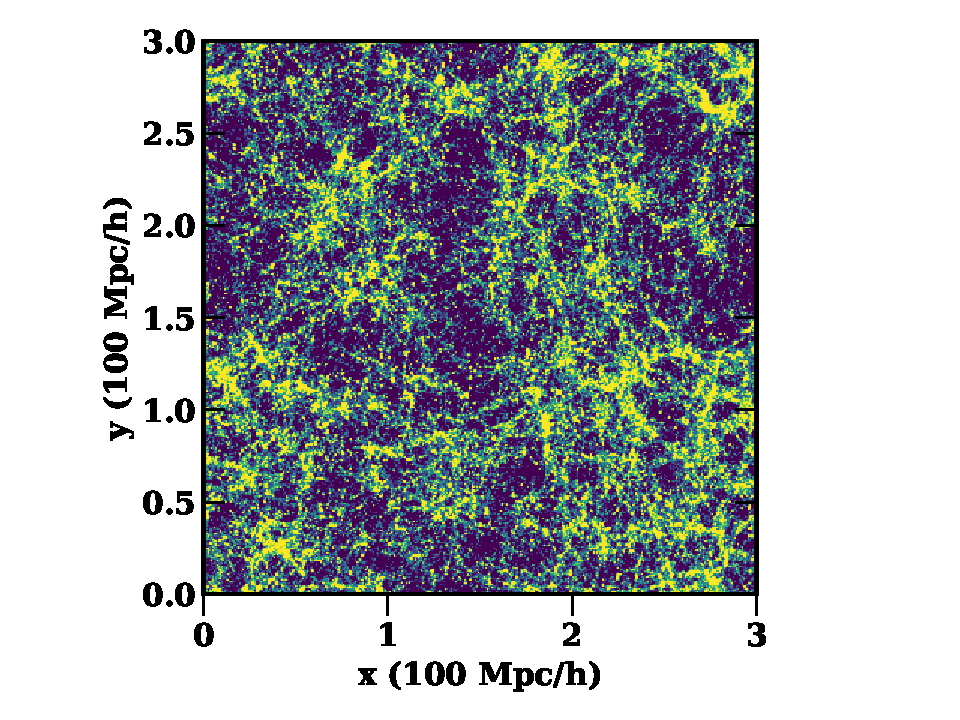
\includegraphics[trim={1.5cm 0 3.3cm 0},clip,width=0.29\textwidth]{nuplots/dens-plt-b300p512nu0_4hyb850t1.pdf}
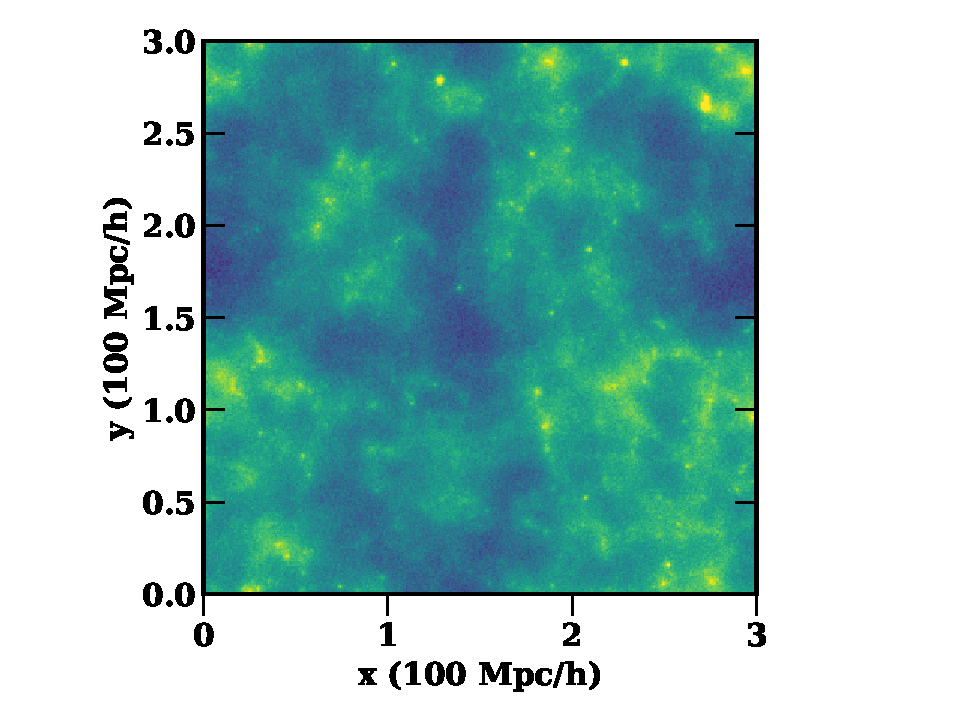
\includegraphics[trim={1.5cm 0 3.3cm 0},clip, width=0.29\textwidth]{nuplots/dens-plt-b300p512nu0_4hyb850t2.pdf}
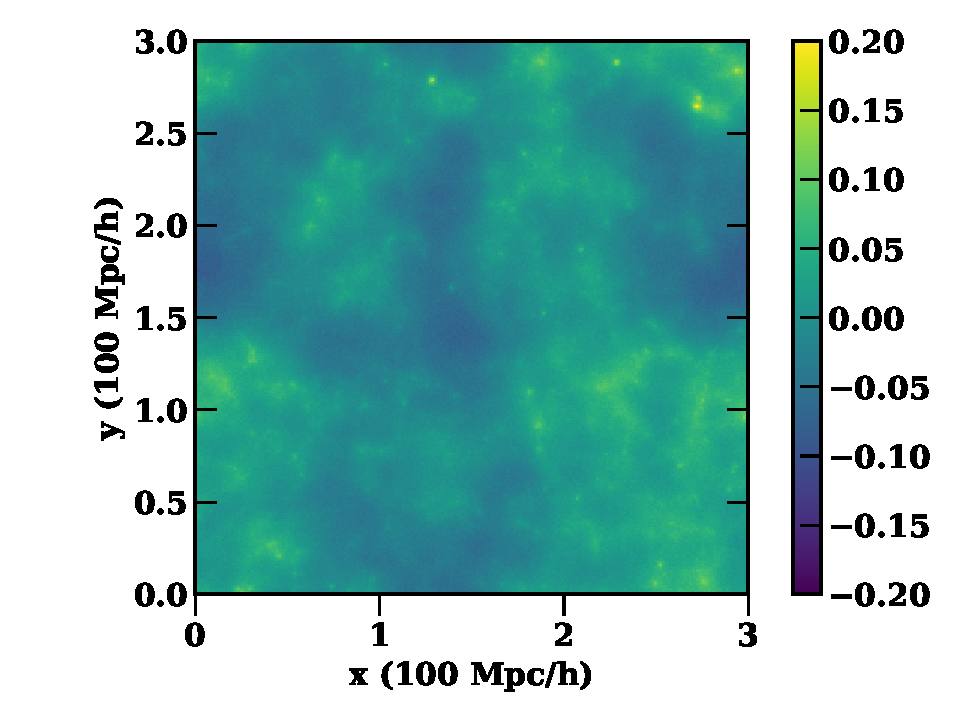
\includegraphics[trim={1.5cm 0 0.5cm 0},clip, width=0.36\textwidth]{nuplots/dens-plt-b300p512nu0_4p1024t2.pdf}
\caption{Projected density plots at $z=0$. \emph{Left}: CDM. \emph{Middle}: Neutrino particles from the hybrid simulation, with unperturbed velocity $<850$ (comoving) km/s. \emph{Right}: Neutrino particles from the pure particle simulation, i.e. including neutrinos from all unperturbed velocities. Colours show $\log (1+ \delta)$ in dimensionless units, where $\delta$ is the over-density projected throughout the box.
  The clustering of the hybrid particles is intermediate between that of the cold dark matter and the particle neutrinos. Colour scale has been truncated for the CDM for clarity. Structures have the same positions in all three panels.
  }
  \label{fig:density_plot}
\end{figure*}

\begin{figure*}
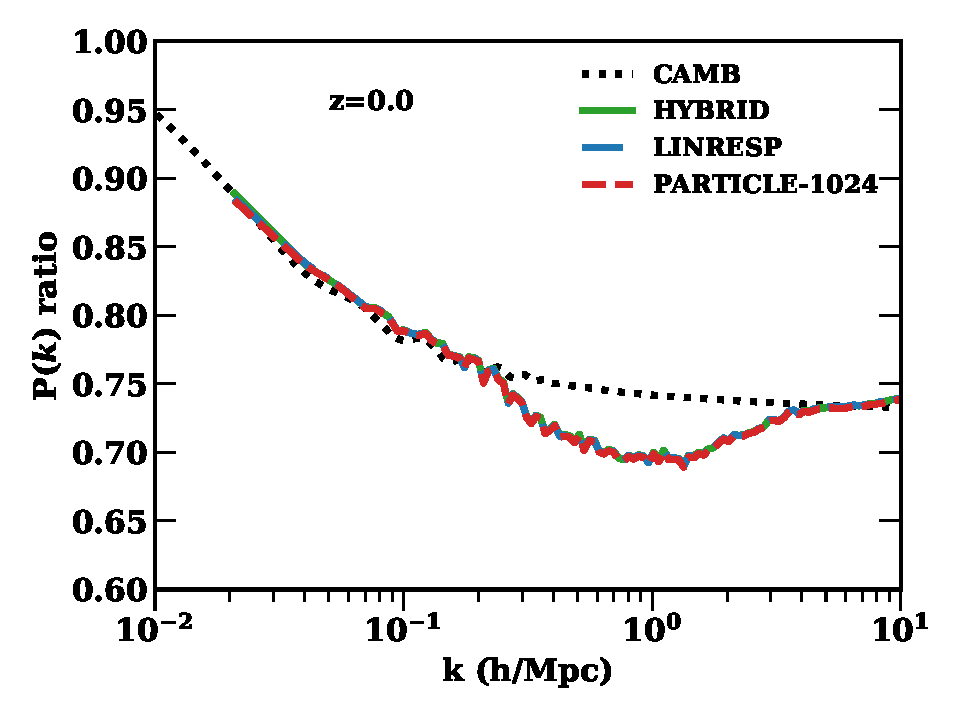
\includegraphics[width=0.45\textwidth]{nuplots/pks_rel-10.pdf}
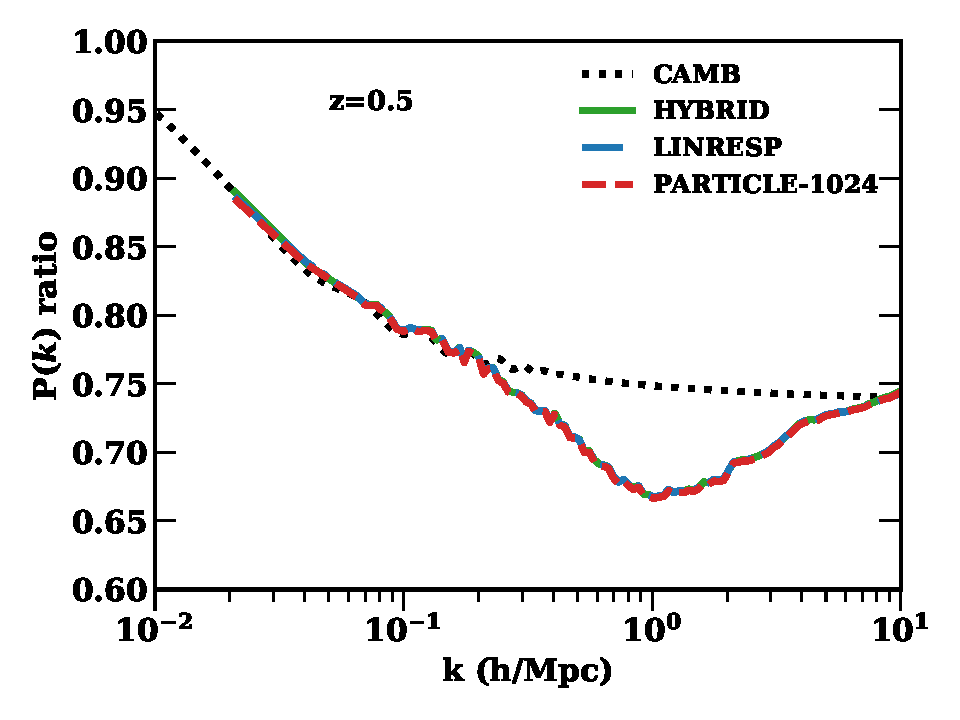
\includegraphics[width=0.45\textwidth]{nuplots/pks_rel-0_66670.pdf}
  \caption{Ratio of matter power spectrum with massive neutrinos ($M_\nu = 0.4$ eV) to matter power spectrum with massless neutrinos. Figure shows hybrid (\texttt{HYBRID}), linear response (\texttt{LINRESP}), and particle (\texttt{PARTICLE-1024}) methods at $z=0$ (left) and $z=0.5$ (right). All three simulation methods agree with $\sim 0.1$\%, %\yah{For the $P(k)$ itself, not the suppression, I presume? To clarify.} \spb{It is the same!}
in agreement with AHB13. Achieving convergence for the particle neutrino method required a large number of neutrino particles, and thus almost an order of magnitude more CPU time, as discussed in Section~\ref{sec:matterpower}.}
  \label{fig:matter_power}
\end{figure*}

\begin{figure}
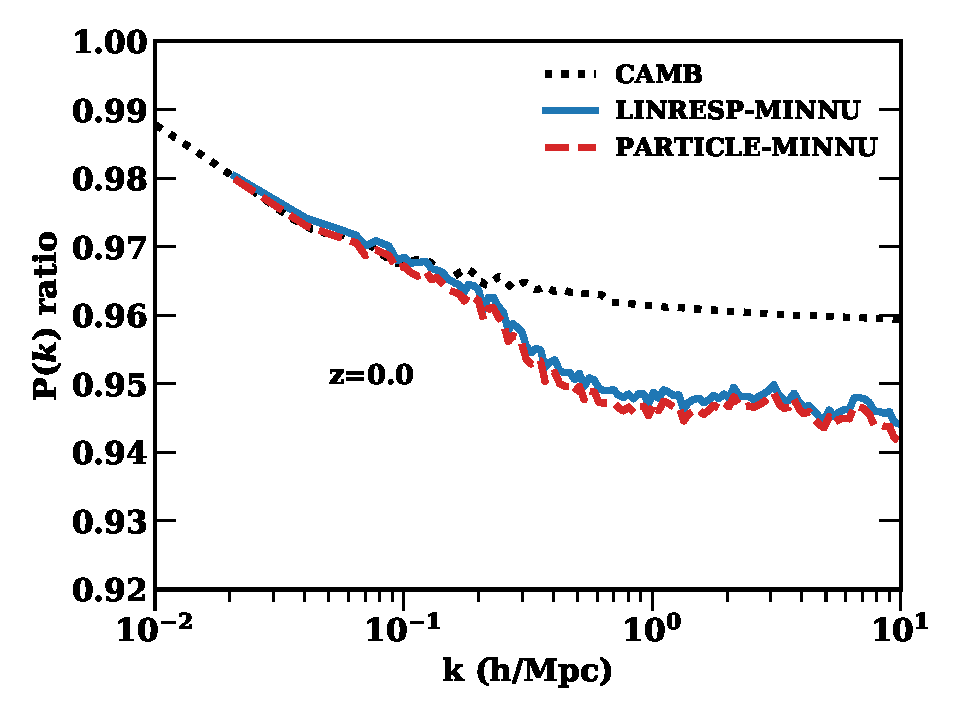
\includegraphics[width=0.45\textwidth]{nuplots/pks_lowmass-10.pdf}
\caption{Ratio of the matter power spectrum with the minimal neutrino mass ($M_\nu = 0.06$ eV) to the matter power spectrum with massless neutrinos at $z=0$. The linear response method (\texttt{LINRESP-MINNU}) and particle method (\texttt{PARTICLE-MINNU}) are shown. At these low masses, the particle method is affected by shot noise. }
\label{fig:minimal_mass}
\end{figure}

Figure \ref{fig:density_plot} shows projected densities for the CDM and neutrino particles from the HYBRID and PARTICLE simulations.\footnote{Projected density plots made using Nbodykit \citep{Hand_2017}.}, in order to give a visual impression of the clustering of the neutrinos and dark matter. The structure of filaments, halos and voids is identical in all three plots, further reinforcing the conclusion of Figure \ref{fig:cross-corr} that the phases of the neutrinos and CDM are highly correlated. The neutrino particles in the hybrid simulation cluster more than in the purely particle simulation, but in both cases less than the CDM. This matches the expected behaviour given their lower initial thermal velocities.

\subsection{Matter Power}
\label{sec:matterpower}

Figure~\ref{fig:matter_power} shows the $z=0$ and $z=0.5$ matter power spectrum for all three neutrino simulation methods: particle, linear response and hybrid. Power spectra are generated using NBodyKit. These three simulations are identical except for the method used to follow neutrino perturbations. In particular, they all use the same cosmological background solution, which includes radiation and massive neutrinos. Figure~\ref{fig:matter_power} shows the ratio of the matter power spectrum in each simulation with massive neutrinos compared to the matter power spectrum from a pure-CDM massless neutrino simulation. We also show the linear theory evolution from CAMB. Validating our new hybrid method, the hybrid and linear response simulation methods produce matter power spectra which are indistinguishable by eye from the particle method, and in fact differ by around $0.1\%$. All simulations agree with CAMB at the $1\%$ level on linear scales, $k < 0.2$ $h$/Mpc.

The particle neutrino simulation contains $1024^3$ neutrino particles, $8\times$ the number of CDM particles. This high particle load increased the computational cost by a factor of $\sim 10$ (note that our simulation includes the short-range gravitational force for the neutrinos). A simulation with $512^3$ neutrino particles underestimated the growth of the matter power spectrum by approximately $1\%$, independently of scale between $z=99$ and $z=49$. AHB13 avoided this discrepancy with linear theory by starting their simulations at a lower redshift ($z=49$), but this leads to inaccuracy in the CDM power spectrum \citep{Heitmann:2010}. This problem is more severe for lower neutrino masses, which would require a lower starting redshift to avoid shot noise. A strength of our hybrid and linear response methods is that the particle neutrinos do not gravitate until late times, when the neutrino power spectrum is no longer shot noise dominated. To demonstrate this explicitly, we performed a hybrid simulation where all neutrinos are followed by the particle component (\texttt{HYBRID-v5000} in Table \ref{tab:simulations}, discussed in Section \ref{sec:nupower}). Thus this simulation is identical to the linear response simulation before the particle switch-on time of $z=1$ and identical to the particle simulation thereafter. Like the simulations shown in Figure \ref{fig:matter_power}, it produces a matter power spectrum in good agreement with CAMB.

Figure \ref{fig:minimal_mass} shows the matter power spectra from simulations with $M_\nu = 0.06$~eV $z=0$. These low neutrino masses will become increasingly important as the upper limit on $M_\nu$ is reduced. We show linear response and particle simulations, but omit a hybrid simulation as for this neutrino mass $ < 4\%$ of the neutrinos have an initial velocity greater than $850$ km/s. The particle simulation neglects the contribution of the two light neutrino species, with masses $0.01$ and $10^{-3}$~eV respectively, as only one neutrino mass state can be followed in a particle simulation\footnote{The background evolution is however identical to the linear response simulation.}. The linear response simulation agrees with linear theory for $k < 0.2$ h/Mpc, further demonstrating that our simulations are able to reproduce the results of linear theory on large scales even for the lowest neutrino mass allowed by oscillation experiments.

For $M_\nu = 0.06$ eV, there is a discrepancy between the particle simulation and the linear response simulation. We have verified that it is the particle neutrino simulation which is discrepant with linear theory. This discrepancy occurs because the particle neutrinos are strongly affected by shot-noise. Our particle simulation used $512^3$ particle neutrinos, matching the number of CDM particles. Ensuring that the neutrino power spectrum is not shot noise dominated at $z=99$ would require $2048^3$ particles for $M_\nu = 0.06$ eV, which is beyond our computational capabilities. The effect of shot noise causes the particle and linear response power spectra to grow steadily more discrepant between $z=9$ and $z=1$, as the particle neutrinos continue to be shot noise dominated even at low redshift. Note that this means that avoiding shot noise with a low starting redshift would cause a large fraction of the nonlinear growth in the CDM to be missed.

\subsection{Halo Mass Functions}
\label{sec:halomass}

\begin{figure}
  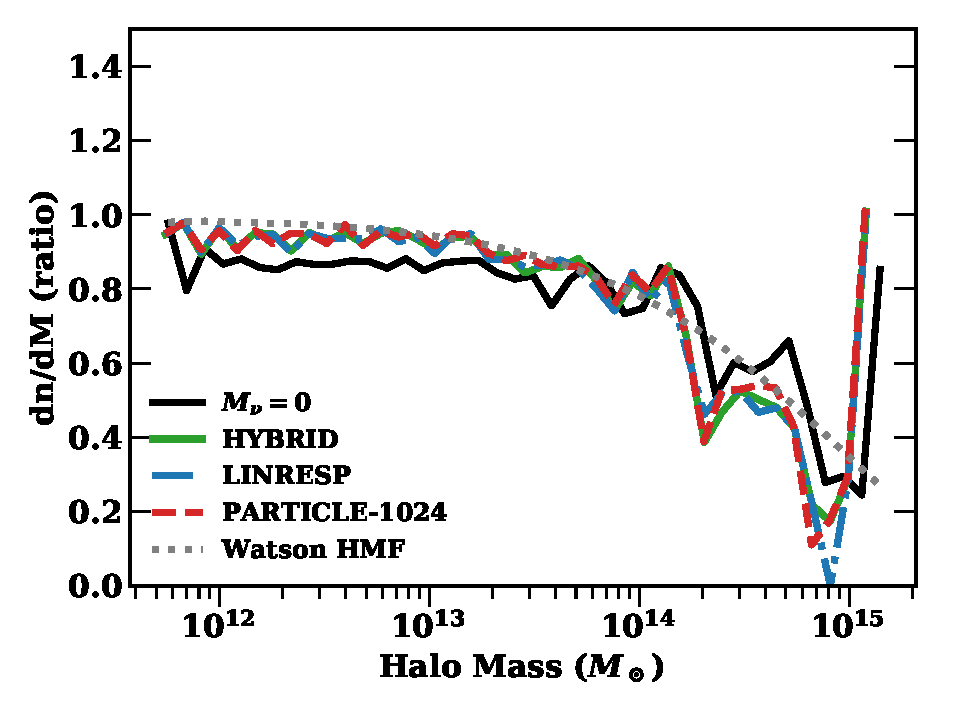
\includegraphics[width=0.45\textwidth]{nuplots/hmf-0_8333.pdf}
\caption{Halo mass functions at $z=0.2$ for our \texttt{PARTICLE-1024}, \texttt{LINRESP} and \texttt{HYBRID} simulations with $M_\nu = 0.4$ eV, as well as the mass function model from \protect\cite{Watson_2013} with parameters matching the massive neutrino model. We normalise by the mass function model with parameters corresponding to $M_\nu = 0$.}
  \label{fig:halomass}
\end{figure}

Figure~\ref{fig:halomass} shows the halo mass functions for our particle, linear response and hybrid simulations. Only CDM particles contribute to the halo mass, for ease of comparison. We show also a mass function model from \cite{Watson_2013}, with $\sigma_8 = 0.7372$, matching the linear power spectrum amplitude for the massive neutrino model. We also set $\Omega_M = \Omega_\mathrm{CDM} + \Omega_b$ (ie, excluding the neutrino component), as recommended by \cite{FVN_2014}. All curves are normalised by a mass function model from \cite{Watson_2013} corresponding to our $M_\nu = 0$ cosmology, with $\sigma_8 = 0.8375$. We choose \cite{Watson_2013} because their calibration simulations use a friends-of-friends mass function with a linking length of $0.2$, as do our simulations. A model is used instead of a simulation to reduce scatter from Poisson noise, and $z=0.2$ is used instead of $z=0$ for the same reason. The simulated mass functions agree very well with each other. Small differences are visible in the largest halo mass bins, where the total number of halos in the box is small and small changes in mass distribution can move a halo to an adjacent bin. There is also a $5\%$ scatter between individual mass bins, due to Poisson noise in the halo catalogue from our finite box. This scatter is the same for all our simulations as we have used the same initial particle realisation in each case. Our simulations agree with the mass function model as well as expected given our small box. We defer a more detailed analysis with more sophisticated halo finders and larger boxes to future work.

\subsection{Clustering of neutrinos}
\label{sec:nupower}

\subsubsection{Correlation of fast neutrinos with the matter field}

As well as the LRA, we make the additional approximation \eqref{eq:phases} in the linear-response integral, so that we need not keep track of the history of the full 3-dimensional matter density field. This approximation implies that fast neutrinos are completely correlated with the dark matter. It is certainly accurate on linear scales, where modes are decoupled. We can further check its consistency with a particle neutrino simulation. Figure~\ref{fig:cross-corr} shows the cross-correlation coefficient between neutrino particles and CDM in a particle simulation and in our new hybrid method, demonstrating that it is indeed close to unity.

We further show the cross-correlation between the CDM and the ``fast'' and ``slow'' neutrino particles. The fast neutrinos, which are always followed using the LRA, are completely correlated with the CDM on all scales where shot noise permits the power spectrum to be reliably computed. This fully justifies Eq.~\eqref{eq:phases} for hybrid simulations. Slow neutrino particles are completely correlated on linear (and mildly non-linear) scales, but uncorrelated on smaller scales, motivating use of a hybrid simulation in simulations concerned with small-scale neutrino overdensities.

\begin{figure}
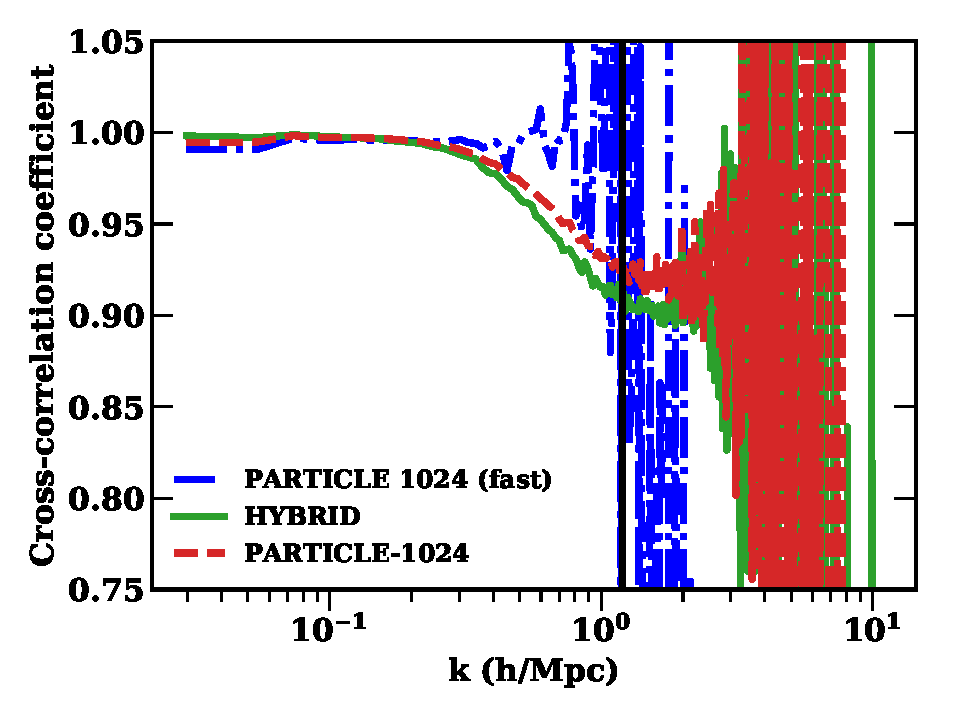
\includegraphics[width=0.45\textwidth]{nuplots/corr_coeff-1.pdf}
  \caption{The cross-correlation coefficient between neutrinos and dark matter using the particle and hybrid simulation methods. The cross-correlation between ``fast'' neutrino particles and dark matter in the particle simulation is shown separately. For the hybrid simulation, only the correlation between the cold dark matter and slow neutrino particles is shown. The vertical black line shows the scale where shot noise dominates the particle simulation.
  }
  \label{fig:cross-corr}
\end{figure}


\subsubsection{Neutrino power spectrum}

\begin{figure*}
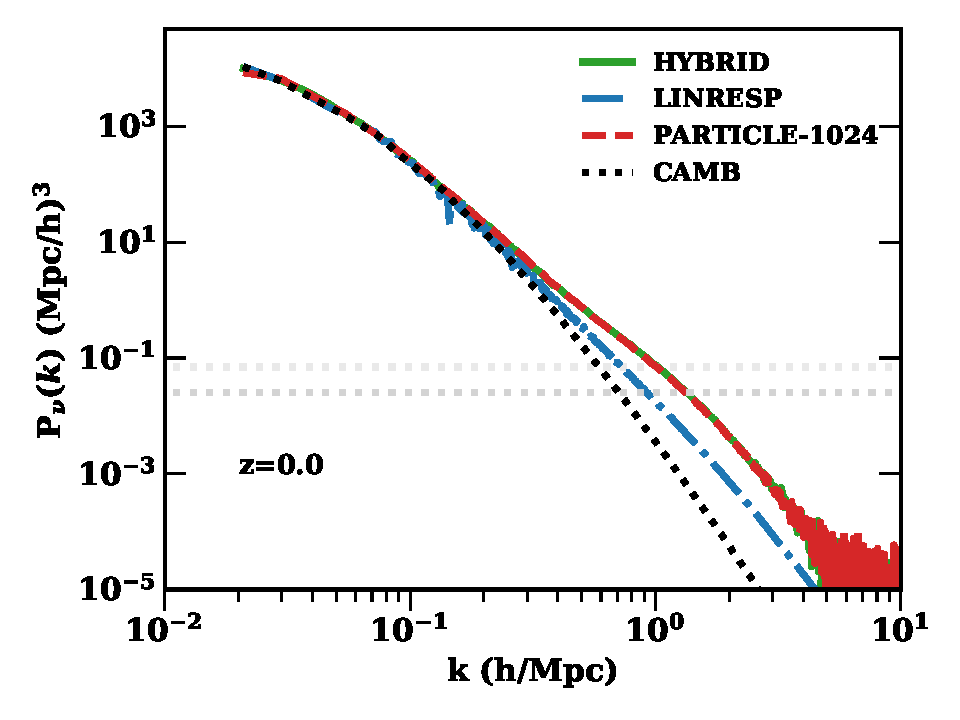
\includegraphics[width=0.45\textwidth]{nuplots/pks-nu-1.pdf}
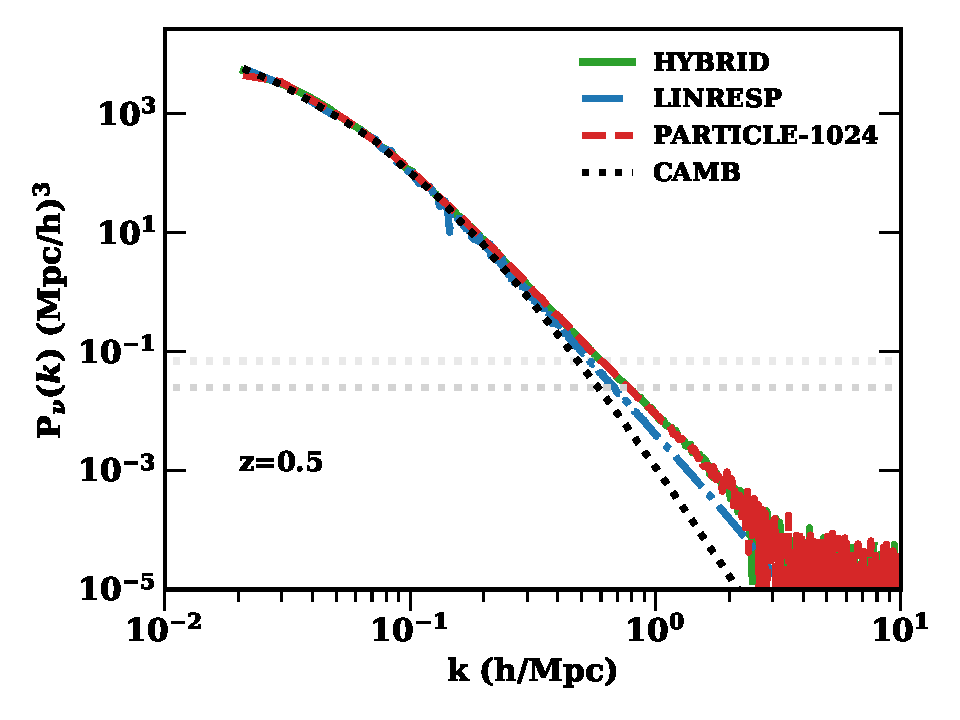
\includegraphics[width=0.45\textwidth]{nuplots/pks-nu-0_6667.pdf}
  \caption{The neutrino power spectrum with massive neutrinos ($M_\nu = 0.4$ eV) for simulations using linear response (\texttt{LINRESP}) hybrid (\texttt{HYBRID}) and particle (\texttt{PARTICLE-1024}) methods. (Left) At $z=0$. (Right) At $z=0.5$. We have subtracted shot noise from the particle and hybrid simulations. The heavier dashed grey curve shows the level of shot noise subtracted from the particle simulation, while the lighter dashed grey curve shows the level subtracted from the hybrid simulation. We show the linear theory neutrino power spectrum from CAMB for comparison. There is good agreement between the hybrid and particle simulation methods.}
  \label{fig:neutrino_power}
\end{figure*}

\begin{figure}
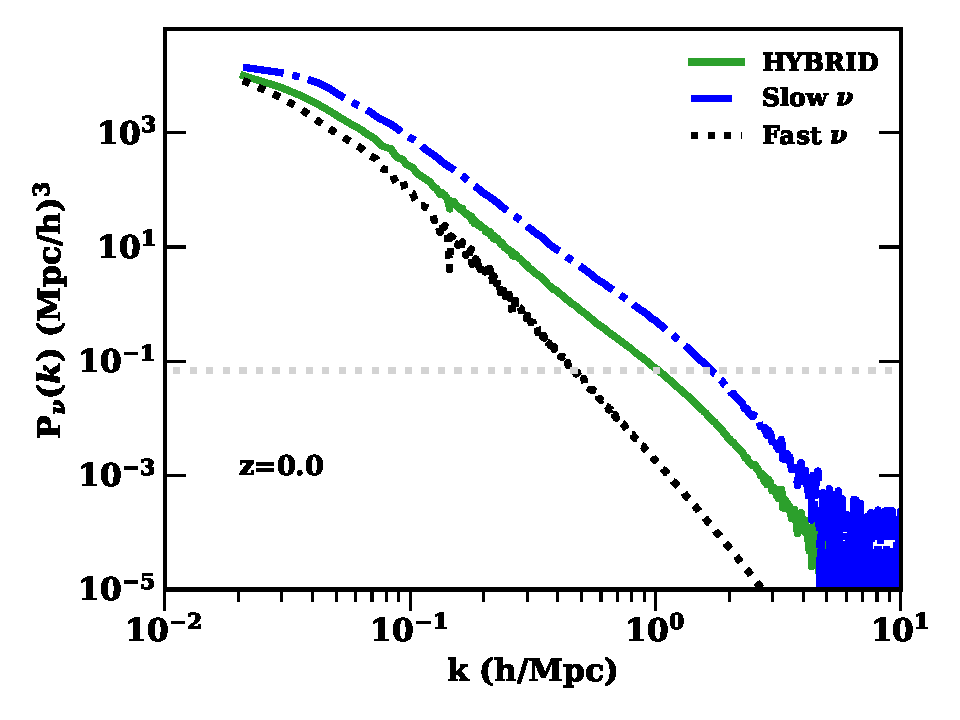
\includegraphics[width=0.45\textwidth]{nuplots/pks-nu-split-1.pdf}
  \caption{The neutrino power spectrum for the hybrid simulation (\texttt{HYBRID}) at $z=0$, split into fast (analytic) and slow (particle) neutrino components. Shot noise has been subtracted at the level shown by the grey line.}
  \label{fig:neutrino_power_split}
\end{figure}

\begin{figure}
  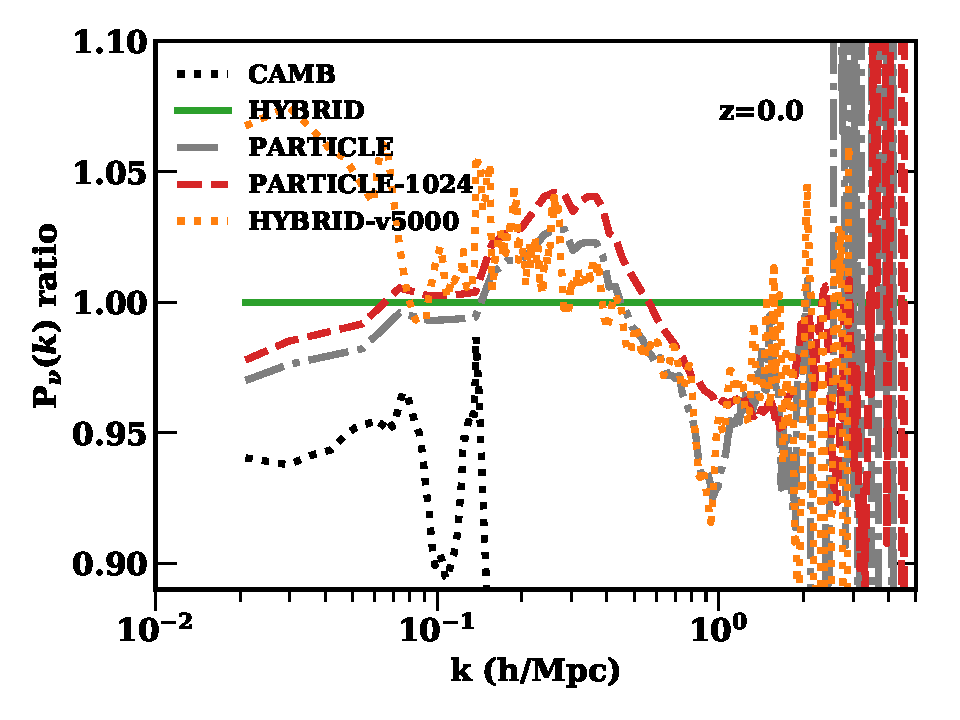
\includegraphics[width=0.45\textwidth]{nuplots/pks_nu_ckrel2-1.pdf}
    \caption{Ratios of neutrino power spectra to the results of the default hybrid simulation. Shown are the default (\texttt{HYBRID}), neutrino particle simulations with $512^3$ neutrino particles (\texttt{PARTICLE}) and $1024^3$ neutrino particles (\texttt{PARTICLE-1024}), and a hybrid simulation where all neutrino mass density is in particles after the switch-on time (\texttt{HYBRID-v5000}). Power spectra have been smoothed with an 11-pt rolling average to reduce scatter and shot noise has been subtracted.}
  \label{fig:hybparticle}
\end{figure}

\begin{figure}
  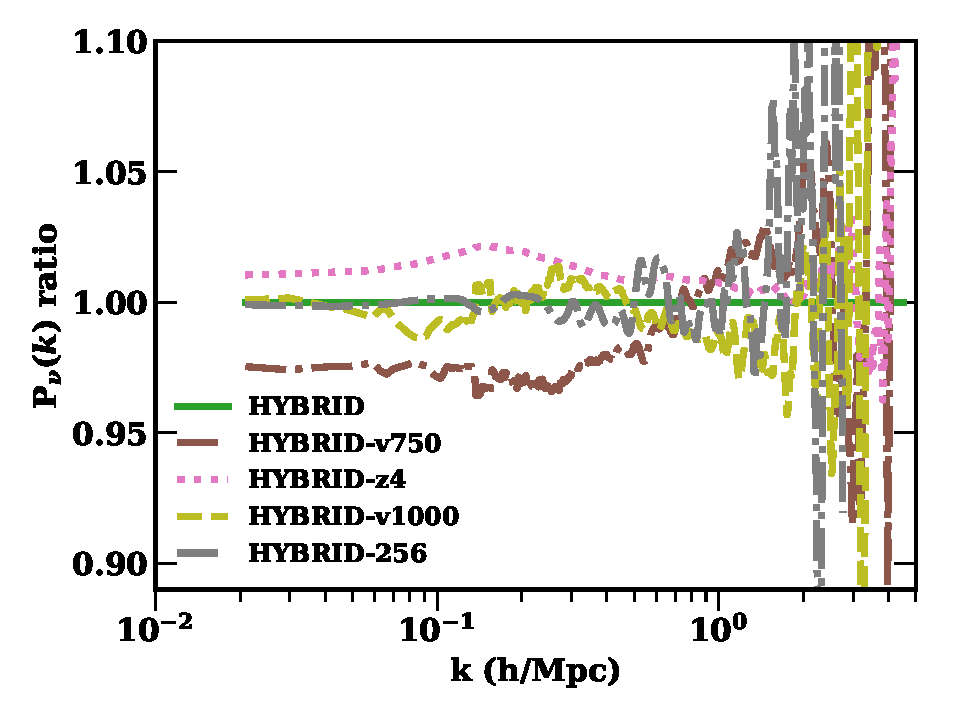
\includegraphics[width=0.45\textwidth]{nuplots/pks_nu_ckrel-1.pdf}
  \caption{Neutrino power spectra from various hybrid simulations compared to the results of the default hybrid simulation (\texttt{HYBRID}). \texttt{HYBRID} has a cut-off velocity of $850$ km/s, a neutrino switch-on time of $z=1$ and $512^3$ neutrino particles. Other simulations shown have neutrino cut-off velocities of $1000$ km/s \texttt{HYBRID-v1000} and $750$ km/s (\texttt{HYBRID-v750}), a switch-on time of $z=4$  (\texttt{HYBRID-z4}) and $256^3$ neutrino particles (\texttt{HYBRID-256}). Power spectra have been smoothed with an 11-pt rolling average to reduce scatter and shot noise has been subtracted.}
  \label{fig:vcrit}
\end{figure}

Figure~\ref{fig:neutrino_power} shows the neutrino power spectrum at $z=0$ and $z=0.5$, demonstrating each of the neutrino simulation methods, as well as the linear theory power spectrum from CAMB. For the hybrid simulation we have computed the total neutrino power spectrum (assuming both neutrino components are completely correlated) as the weighted sum of the power spectrum of the fast and slow components $P^{1/2}_\nu = f_\mathrm{fast} P^{1/2}_\mathrm{fast} + f_\mathrm{slow} P^{1/2}_\mathrm{slow}$, where $f_\mathrm{fast} + f_\mathrm{slow} = 1$. Figure~\ref{fig:cross-corr} shows that this is a good approximation for $k < 0.5$ h/Mpc. For $k > 0.5$ h/Mpc, the slow neutrinos contribute $> 95\%$ of the total power, so that a $10\%$ decorrelation would over-estimate the neutrino power by only $0.5\%$. Figure~\ref{fig:neutrino_power_split} shows the neutrino power spectra for each individual component, showing the increased clustering for the slow neutrinos.

Neutrino particle shot noise has been subtracted from both the particle and hybrid simulation. The shot noise for the hybrid simulation is $P_\mathrm{shot} = 0.346^2\times (300 /512)^3 $ (Mpc/$h)^3$, where the factor of $0.346$ is due to the reduced matter density in particle neutrinos. The particle simulation has $P_\mathrm{shot} = (300 /1024)^3$ (Mpc/$h)^3$. In both simulations, the neutrino power is recoverable even two orders of magnitude below the shot noise level, indicating that there is little structure formation arising purely from neutrino shot noise.

%The hybrid approach is converged at a higher nominal level of shot noise, due to lower thermal velocities.

At $z \geq 1$ all three methods are in good agreement, consistent with the results of AHB13. At $z = 0$ and $z=0.5$, the hybrid neutrino simulation and neutrino particle simulation are in good agreement. However, the linear response method shows reduced power on small scales. This is in agreement with the expectations from Section~\ref{sec:hybrid} and demonstrates that our hybrid method indeed resolves the discrepancy between the linear response method and the particle method. Figure~\ref{fig:hybparticle} compares the neutrino power spectrum from the particle and hybrid methods in more detail. There are two interesting features: a deficit of power in the particle simulations at $k=1$ $h$/Mpc, and an increase in power at $k=0.2$ $h$/Mpc. The first is consistent with being due to the increased mass resolution in the hybrid method, which would lead to increased power on small scales. Note that the feature is smaller in the higher resolution particle simulation. The origin of the second is unclear. We also show a hybrid simulation (\texttt{HYBRID-v5000}) where all neutrino mass density is in particles. This simulation evolves like a particle simulation after the neutrino switch-on time of $z=1$, but is identical to a linear response simulation before that. Although the comparison is noisy, \texttt{HYBRID-v5000} does not exhibit the same increase in power at $k=0.2$ $h$/Mpc. This suggests it is an effect which occurs before the neutrino switch-on time; either true non-linear neutrino structure formation which is missed because the neutrino particles are not yet actively gravitating, or artificial structure formation induced by shot noise. Overall, however, the differences between the particle and hybrid methods are not larger than $5\%$, which we consider an acceptable degree of convergence for a quantity with is less than $1\%$ of the total matter density.

Figure~\ref{fig:vcrit} shows how the neutrino power spectrum from hybrid simulations depends on the model parameters. We show simulation outputs at $z=0$, but have checked that higher redshifts produce similar results. In particular, we have varied the neutrino switch-on time, the critical neutrino velocity and the number of neutrino particles (and thus the level of shot noise). The total matter power spectra for all these simulations agreed to $0.5\%$ for $k < 5$ h/Mpc. Increasing the critical neutrino velocity to $v_\mathrm{crit} = 1000$ km/s (\texttt{HYBRID-v1000}) from $850$ km/s did not alter the neutrino power spectrum by more than $1\%$, as all non-linear growth occurs in neutrinos with unperturbed velocities less than $850$ km/s. By contrast, when the critical velocity is reduced to $750$ km/s (\texttt{HYBRID-v750}), the neutrino power spectrum is reduced by $3\%$, indicating moderate non-linear growth in these velocity bins. These results confirm the calculations of Section~\ref{sec:hybrid}.

The \texttt{HYBRID-z4} simulation changed the initial neutrino switch-on time from $z=1$ to $z=4$. There is a moderate discrepancy, with a $z=4$ switch-on time leading to $1-2\%$ more power than a $z=1$ switch-on time. As with the particle simulation, the reason for this is unclear. It could be due to the inclusion of non-linear power at $z>1$, or it could be due to residual shot noise. In any case the effect is relatively small. Finally, we show \texttt{HYBRID-256}, a hybrid simulation where the neutrino particle load has been decreased by a factor of $8$, to $256^3$. This changed the neutrino power spectrum by less than $1\%$ and shows that we are well converged with respect to mass resolution and neutrino shot noise at $z < 1$.
The effects of changing the hybrid simulation parameters are not large, and our simulations appear well converged.

\section{Conclusions}
\label{sec:conclusion}

We have extended the linear-response neutrino simulation method from \cite{AHB} to better account for non-linear growth in the neutrino component and thus reproduce the non-linear neutrino power spectrum as well as the non-linear matter power spectrum.
Our improved method is a hybrid: initially fast-moving neutrinos are followed as before using a linear response method, while initially slow-moving neutrinos, which can be captured by CDM halos, are followed using particles at late times. Neutrinos are followed analytically at early times, allowing the hybrid method to avoid the impact of shot noise with a much lower particle load. We show that our new hybrid method reproduces the non-linear matter power of the linear response simulations, as expected from \cite{AHB}, while also reproducing the significantly large neutrino power spectrum seen in a converged particle simulations at $z=0$. We show that the hybrid method agrees well with CAMB when structure growth is linear. Since only a fraction of the neutrino matter density is followed by neutrinos, we show that converged results can be obtained with a relatively small neutrino particle load. Our simulation code is publicly available, both integrated into the simulation code MP-Gadget and as a series of patches to Gadget-2 \footnote{\url{https://github.com/sbird/kspace-neutrinos}}.

% In summary, our new hybrid method agrees well with CAMB on linear scales, for both neutrino and matter power spectrum. It reproduces the non-linear matter growth function of both particle and linear response simulations, and the non-linear neutrino growth seen in the particle simulation, with somewhat higher resolution.

Most simulators wishing to compare to observational surveys can use the linear response method, as it is computationally efficient and still reproduces well the properties of the total matter density, which are the directly observable quantities. However, for simulators wishing instead to investigate the structure of the neutrino component, our hybrid method provides much improved accuracy. Simulations using our method could be used to investigate, for example, the distribution of neutrino matter around collapsed objects \citep{FVN_2013}, neutrino wakes \citep{Inman_2015}, the neutrino bispectrum \citep{Furhrer_2015} or the distribution of massive neutrinos in cosmic voids \citep{Banerjee_2016}. We showed that a neutrino switch-on redshift $z=1$ and a critical neutrino velocity of $850$ km/s include the majority of non-linear neutrino velocity shells, as well as showing good convergence properties for $M_\nu \leq 0.4$ eV.

Our linear response simulations have computational costs similar to pure cold dark matter simulations. Our hybrid simulations required about twice the computational time of a linear response simulation, for a neutrino particle load equal to that of the CDM. This compares well to the extra cost of the particle simulations, which was a factor of $10$ for a fully converged simulation. Simulators may consider further reducing the computation cost of the hybrid simulations by reducing the neutrino particle load below that of the CDM. We found that in our simulations a particle load of $256^3$, $1/8$th that of CDM, gave identical results for the neutrino power spectrum. Our hybrid linear response-particle simulations are thus substantially faster than pure particle simulations, allowing simulation suites to sample a cosmological parameter space with massive neutrinos substantially more finely.

Finally, we note that cosmological surveys have now reached a level of sensitivity where even the minimal neutrino mass can substantially alter derived parameters \citep{Calabrese_2017}, and thus the inclusion of massive neutrinos (and radiation in the background) should become standard for all simulators. For these mass ranges including the neutrino mass hierarchy is important, and removing all neutrino particle shot noise prohibitively expensive. Both problems are avoided by our linear response or hybrid methods.

\section*{Acknowledgements}

We thank Arka Banerjee for sharing simulation data. We thank Jeremy Tinker and Derek Inman for useful discussions.
This research project was conducted using computational resources
at the Maryland Advanced Research Computing Center (MARCC). SB was supported by NASA through
Einstein Postdoctoral Fellowship Award Number PF5-160133.

\appendix

\section{Manual}
\label{sec:manual}

In this Appendix, we briefly describe the parameters of the linear response neutrino method. A similar description may be found in the README of the code repository: \url{https://github.com/sbird/kspace-neutrinos/}. Our neutrino integrator has been altered to be a stand-alone module, largely independent of the underlying N-body code. To aid integration, we have included copious comments and unit tests. A script is provided in the repository which downloads and patches a fresh copy of Gadget-2 to include massive neutrinos: the ``apply-patches'' script in the gadget-2 subdirectory.

Table \ref{tab:parameters} shows a list of the required parameters, as well as brief descriptions. The number of extra parameters required is small. Three parameters are required to specify the initial power of the neutrino component, using a CAMB or CLASS transfer function file. Three parameters are required to specify the masses of the three active neutrino species.
There is a global switch enabling the hybrid neutrino model. Note that the matter power spectrum is extremely well converged by the linear response method alone. The hybrid neutrino model includes two additional parameters: the critical velocity below which neutrinos are particles, and the neutrino switch-on time, after which neutrinos are actively gravitating. The default values of these parameters are justified in Section~\ref{sec:hybrid}, and may be altered as desired for the problem of interest.
Note that the critical velocity used in MP-Gadget should match that set in the initial conditions code. In this work we also used a neutrino particle load $8$ times smaller than the CDM particle load, which was sufficient to produce a converged neutrino power spectrum on the scales of interest.

%TABLE OF SIMULATIONS.
\begin{table*}
\begin{center}
\begin{tabular}{|l|l|}
\hline
    Parameter & Description \\
\hline
KspaceTransferFunction   & CMB transfer functions, used to compute the neutrino the neutrino integration. \\
TimeTransfer             & Scale factor of the CMB transfer functions. \\
InputSpectrumUnitLengthincm   & Units of the CAMB transfer function in cm. \\
MNue, MNum, MNut &  Three neutrino masses. The measured mass splittings are not enforced. \\
Vcrit            & Critical velocity below which the neutrinos are particles, if hybrid neutrinos are on. \\
NuPartTime       & Scale factor at which the particle neutrinos start to gravitate, if hybrid neutrinos are on. \\
HybridNeutrinosOn       & Switch to enable hybrid neutrinos. \\
\hline
\end{tabular}
\end{center}
\caption{Table of code parameters, with brief descriptions.}
\label{tab:parameters}
\end{table*}

As documented in \cite{Springel_2005} and the Gadget-2 manual, Gadget-2 and some versions of Gadget-3 output snapshots mid-timestep. This is implemented by drifting all particles (even those not currently active) to the desired output time. However, particles are not kicked to update their momenta, so that the output particle velocities are those from the last active timestep. For neutrino particles, whose clustering is intimately tied to their total momentum, restarting from a snapshot using Gadget-2 or later will introduce an error in the $z=0$ power spectrum. Gadget-2 simulators should restart their simulations, if necessary, from restart files. This does not apply for MP-Gadget, which we have modified so that snapshots always occur at the end of a PM timestep, when all particles are active. Finally, when using Gadget-3 and neutrino particles, the force tree should be rebuilt every timestep, as otherwise the neutrino thermal velocity causes the tree nodes to become extremely large.





\section{Initial Conditions}
\label{sec:initcond}

% \begin{figure*}
% 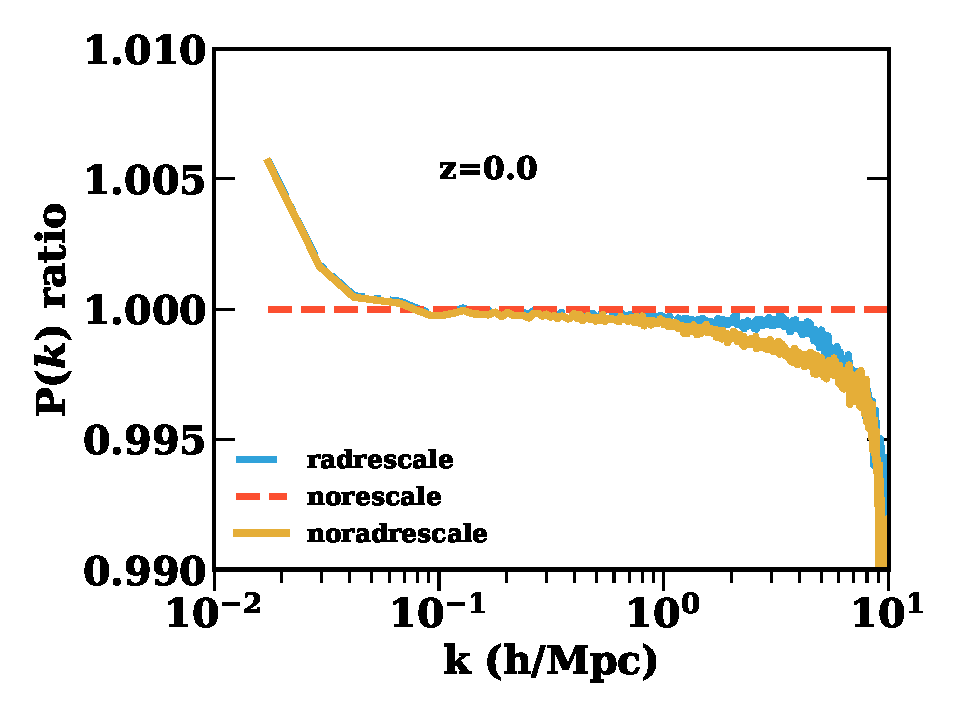
\includegraphics[width=0.45\textwidth]{icplots/pks_rel-1.pdf}
% 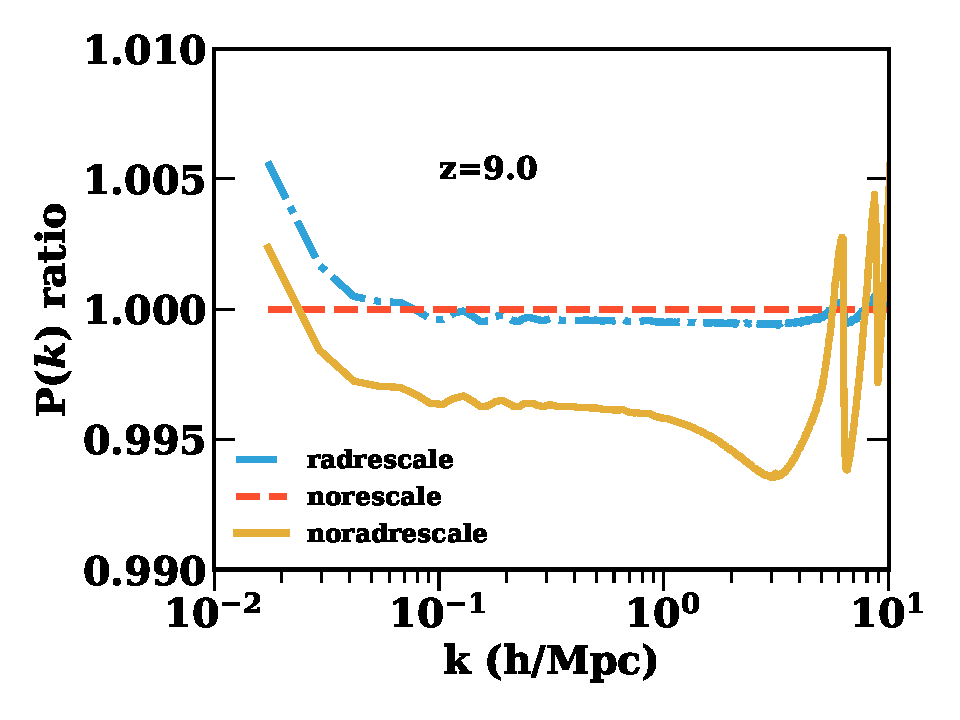
\includegraphics[width=0.45\textwidth]{icplots/pks_rel-0_1.pdf}
% % \includegraphics[width=0.45\textwidth]{icplots/pks_camb-1.pdf}
%   \caption{The ratio between matter power spectra from three simulations with different initial conditions.
%   These are initialized respectively using the $z=99$ (norescale) transfer function,
%   the scaled $z=0$ transfer function (radrescale), and the $z=0$ transfer function
%   scaled and evolved neglecting radiation density (noradrescale). Power spectra are normalised to the norescale simulation.
%   (Left) At $z=0$. (Right) At $z=9$.}
%   \label{fig:rescaling}
% \end{figure*}

In this Appendix, we detail improvements to the accuracy of our simulation initial conditions since AHB13.
Following Lagrangian perturbation theory \citep{Zeldovich_1970, Scoccimarro_1998},
the particle velocities and displacements are related by:
\begin{equation}
v(k) = a H(a) \frac{d \log D(a)}{d \log a} \delta(k)\,.
\label{eq:vel_prefac}
\end{equation}
$D(a)$ is the linear growth function and $H = \dot{a}/a$ the Hubble function.

In AHB13, the Hubble function used in Eq.~\eqref{eq:vel_prefac}
neglected radiation density. Furthermore, following \cite{Bouchet:1995}, we
approximated the derivative of the linear growth function, $\frac{d \log D(a)}{d \log a}$, by
\begin{equation}
\frac{d \log D(a)}{d \log a} \approx \left(\frac{\Omega_M a^{-3}}{\Omega_M  a^{-3} + \Omega_\Lambda}\right)^{0.6} \approx 1\,.
\end{equation}

This approximation is valid in matter domination, but again neglects the radiation density,
which becomes non-negligible at $z > 50$. Both of these approximations are especially notable
when simulating massive neutrinos, because at high redshift neutrinos are slightly relativistic,
and thus the background density depends slightly on the neutrino mass. In practice the error
induced by each approximation partially cancels, leaving an under-estimation of the effect of
massive neutrinos on structure formation by $\sim 2 \%$, visible in, for example,
Figure 4 of AHB13\footnote{We thank Francisco Villaescusa-Navarro for first pointing these problems out to us.}.

In the simulations presented here we use both the full Hubble function
and obtain $\frac{d \log D(a)}{d \log a}$ by numerically solving
the linear growth equation \citep{Peebles:1993}:
\begin{equation}
\frac{d}{da}\left(a^3 H(a) \frac{d D(a)}{da}\right) - \frac{3}{2} \frac{H_0^2\,D(a)}{a^2 H(a)} \left(\Omega_\mathrm{CDM} + \Omega_\mathrm{b}\right)= 0\,.
\end{equation}
The initial conditions for this differential equation are set at $z \gg 100$ corresponding
to the growing mode in a matter-radiation universe \citep{Groth:1975}:
\begin{equation}
  D(a_i) = \Omega_\gamma + \Omega_\nu + \frac{3}{2} \left(\Omega_\mathrm{CDM} + \Omega_\mathrm{b}\right) a_i\,.
\end{equation}
The above is appropriate for our simulations, because our simulation box size is smaller than the neutrino free-streaming scale at our initial redshift, and thus neutrinos do not cluster. For simulations which probe large scales the scale-dependent growth rate should be used, as in \cite{OLeary_2012, Zennaro_2017}. We have checked explicitly that for our box size the scale-dependent and scale-independent growth rates are the same and since the simulations reported here were performed we have switched our initial conditions generator to using scale-dependent growth rates computed by numerically differentiating synchronous gauge transfer functions.

Our initial conditions are generated using the CAMB CDM + baryon transfer function at $z=99$. An alternative is to generate initial conditions
using the $z=0$ transfer function, scaled to the initial redshift by the (sub-horizon) linear growth function, $D(z_\mathrm{ic})$. This can be used to account for background radiation density, if radiation is not included in the background evolution, or for radiation perturbations and other relativistic effects on the scale of the horizon at $z=99$ \citep{Zennaro_2017}. For the case of massive neutrinos implementing the rescaling is scale-dependent and requires computing equations for a two-fluid system, as neutrinos are no longer free-streaming on the scales of interest at $z=0$.

For our simulations background radiation is included and the simulation box is less than the horizon size. Moreover, we initialize our velocities using the time derivative of the synchronous gauge density perturbations, corresponding to the N-body gauge \cite{Fidler_2015, Valkenburg_2017}. In this gauge relativistic effects vanish at first order and super-horizon evolution is modelled correctly, providing we start in matter domination. The $z=0$ matter power spectrum rescaled to $z=99$ correctly accounting for neutrinos is thus identical to the $z=99$ matter power spectrum we use for initialization, making the rescaling procedure trivial.

Any non-trivial rescaling would introduce an error in the $z > 0$ power spectra due to the mismatched growth functions, which increases at higher redshift. We found that for a massless neutrino simulation which does not include radiation in the background evolution this error is $0.5\%$ on linear scales at $z=9$ and moderately larger on non-linear scales. This (small) error is easy to avoid by using the correct background evolution, as we have done in this paper.

\label{lastpage}

\bibliography{neutrinos}

\end{document}
